\documentclass[12pt,a4paper,ruledheader, capchap]{abnt}
\usepackage{hyperref} % para ter hyperlinks no documento
\usepackage[utf8]{inputenc} %hifenizacao
\usepackage[center]{caption2} 
\usepackage[brazil]{babel} %acentuacao para o idioma pt br
\usepackage[T1]{fontenc}
\usepackage{subfigure} % para subfiguras
\usepackage[pdftex]{graphicx}
\usepackage{abnt-alf} %pacote abnt
\usepackage{latexsym}
\usepackage{multirow}
\usepackage{float}
\usepackage{longtable}
\usepackage{amsmath}
\usepackage[alf]{abntcite}
\usepackage{tabularx} % para tabelas grandes

%altera fonte do capitulo
\renewcommand{\ABNTchapterfont}{\bfseries} 
%altera tamanho da fonte do capitulo
\renewcommand{\ABNTchaptersize}{\Large}
%altera tamanho da fonte dos apendices 
\renewcommand{\ABNTanapsize}{\Large}


\begin{document}
\setcounter{page}{0}
\tableofcontents
%\chapter{Fundamentação das Máquinas de vetores de suporte} \label{cap:svm}

As Máquinas de Vetores de Suporte (SVM, do inglês \textit{Support Vector Machine}) surgiram com o emprego da teoria da aprendizagem estatística, desenvolvida pelo pesquisador Vladimir Vapnik e colaboradores \cite{Vapnik1998}. Mais precisamente, a SVM é uma implementação do método de minimização estrutural de risco. Este método busca minimizar o erro do conjunto de treinamento, juntamente com o erro do conjunto de teste. O objetivo da SVM é criar um bom meio de aprendizagem que separe grandes dimensões através de um hiperplano, de tal maneira que as margens sejam ótimas, que seja computacionalmente eficiente e capaz de lidar com amostras de tamanhos da ordem de 100 000. Nesta Capitulo será revisada a teoria básica para a construção da SVM. Na Seção \ref{S1}, a SVM será introduzida como parte do conjunto de métodos de aprendizagem dentro das redes neurais, serão apresentados os princípios básicos de redes neurais necessários, para a compreensão deste capitulo. Na Seção \ref{S2}, vamos ver os paradigmas de aprendizagem e situaremos a condição da SVM ante a estes paradigmas. Em seguida veremos na Seção \ref{S3} a teoria que originou a criação da SVM. Na sequência será revisado na Seção \ref{Teot}, conceitos de otimização necessários para a solução da SVM. E por fim será visto a teoria da SVM primeiramente para os casos onde os dados são linearmente separáveis Seção \ref{cap:svm:svm-l}. Então para os casos onde os dados não separados linearmente Seção \ref{cap:svm:svm-nl}. Finalizando o capitulo com os métodos utilizados para a solução da SVM Seção \ref{spq}.

\section{Introdução as Redes Neurais Artificiais} \label{S1}
As Redes Neurais Artificiais (RNA do inglês \textit{Artificial Neural Networks}) foram motivadas a partir funcionamento do  cérebro, este é um complexo sistema constituído de aproximadamente duzentos bilhões de células que pode computar problemas com características não triviais, como computações em paralelo, ou problemas não lineares. A estrutura do cérebro é organizada em subunidades chamadas de neurônios, que são responsáveis pelos cálculos realizados no cérebro \cite{Haykin99}.

Os neurônios se interligam a fim de realizar tarefas como: o reconhecimento de padrões; percepção; e coordenação motora. Eles têm a capacidade de adaptar-se ao ambiente, através de estímulos enviados para eles. A Figura \ref{fig:neuronio-nat} apresenta um neurônio natural.

\begin{figure}[htb]
	\centering
	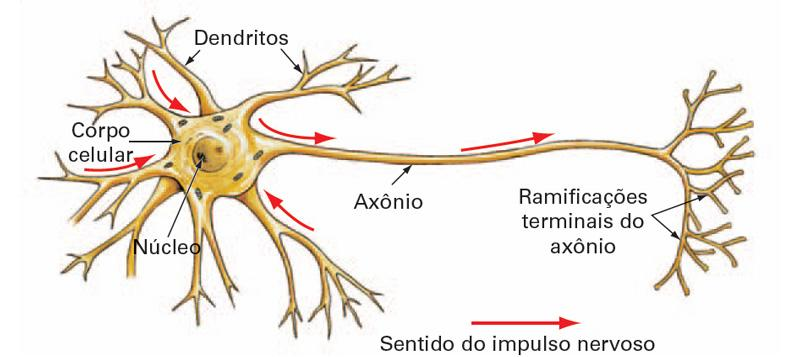
\includegraphics[scale=0.5]{./figuras/neuronio-nat.jpg}
	\caption{Neurônio natural}
	\label{fig:neuronio-nat}
\end{figure}

Com base no comportamento dos neurônios biológicos, pesquisadores modelaram matematicamente o neurônio. Um neurônio é uma unidade de processamento fundamental em uma RNA. A representação dele em forma de diagramas pode ser vista na Figura \ref{fig:neuronio_artificial}.

\begin{figure}[htb]
	\centering
	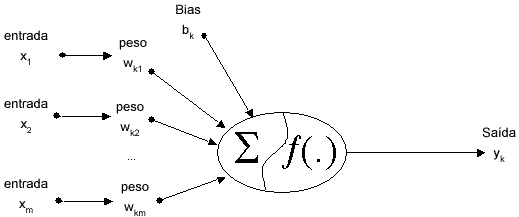
\includegraphics[scale=0.8]{./figuras/neuronio_artificial.jpg}
	\caption{Neurônio artificial (Adaptado de \cite{Haykin99})}
	\label{fig:neuronio_artificial}
	%http://www.lncc.br/~labinfo/tutorialRN/frm1_neuronio.htm
\end{figure}

Podemos observar pela figura um conjunto de ligações sinápticas e seus respectivos pesos $w$, este é um vetor, ligando os dados do também vetor de entrada $x$ ao somador e $m$ é o numero de dados. É realizado o produto entre os vetores $x$ e $w$ e o resultado é aplicado ao somador. A soma de todas as entradas é processada por uma função de saída $f(.)$, também conhecida como função de ativação, que limita a amplitude de saída de um neurônio. As funções de saída mais comuns são: função limiar; função sigmóide; e função hiperbólica. A função Limiar apresentada na Equação \ref{svm:E0} merece atenção devido ela ser adequada às SVMs.

\begin{equation} \label{svm:E0}
y = \left\{\begin{matrix}
+1, & se\ F & \left( \sum_{i=0}^{m=1} x_{i}w_{i} + b \right) > 0 \\ 
														       \\		
-1, & se\ F & \left( \sum_{i=0}^{m=1} x_{i}w_{i} + b \right) < 0
\end{matrix}\right.
\end{equation}

O parâmetro externo $b$ é denominado bias, ele aumenta ou diminui o número de grau de liberdade no modelo, o que permite a rede uma capacidade maior de se ajustar.

Existem diversos algoritmos baseados no modelo de neurônio apresentado, como o Perceptron, Perceptrons de Múltiplas Camadas, e as SVMs. A combinação dos neurônios nas SVMs é mostrada na Figura \ref{fig:SVM-RNA}. O SVM é uma RNA com duas camadas, na camada de saída há apenas um neurônio que é responsável pela construção da função linear no espaço.

\begin{figure}[htb]
	\centering
	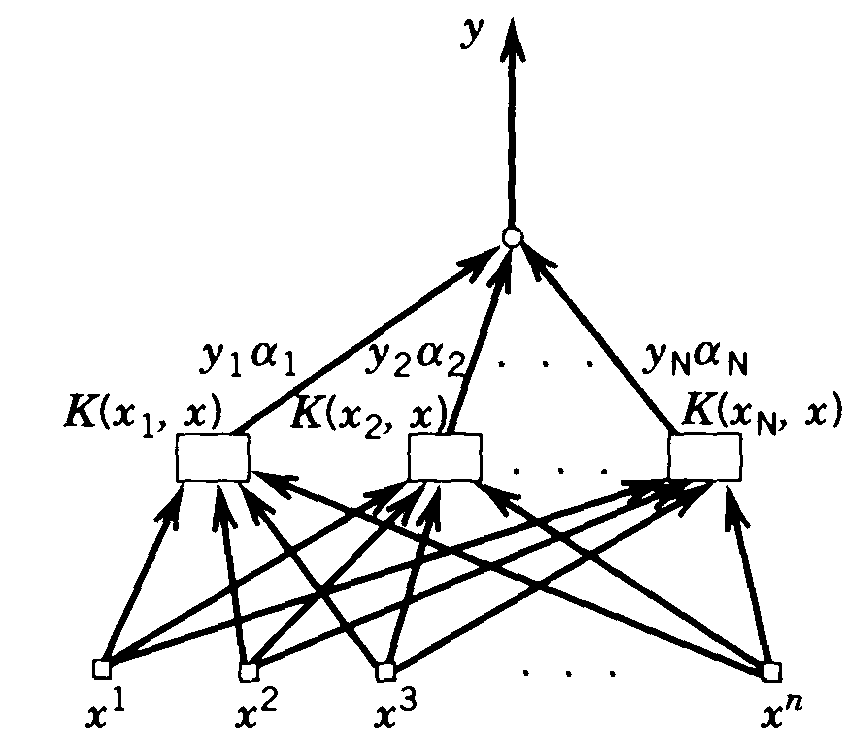
\includegraphics[scale=0.5]{./figuras/SVM-RNA.png}
	\caption{Representação da rede de neurônios do SVM \cite{Vapnik1998}}
	\label{fig:SVM-RNA}
\end{figure}

\section{Conceitos básico de aprendizagem } \label{S2}

A aprendizagem de máquina (AM) é o processo no qual algoritmos desenvolvidos para o computador são capazes de obter conhecimento sobre um determinado problema a partir de resultados observados numa parte desse problema, e gradativamente melhorar o desempenho da aprendizagem. O sistema de aprendizagem é estimulado por um ambiente, este estímulo resulta em modificações em sua estrutura interna e por fim na maneira que o sistema vai responder ao ambiente. As técnicas desenvolvidas para a AM tem como princípio a inferência indutiva. A inferência indutiva para aprendizagem pode ser dividida em três grupos: aprendizagem supervisionada (com professor), aprendizagem por reforço (sem professor)  e aprendizagem não-supervisionada (sem professor).

Na aprendizagem supervisionada temos a figura de um professor, que é um individuo com conhecimentos sobre o ambiente e consequentemente dos exemplos de entrada do sistema de aprendizagem, este conhecimento é na forma: entrada e saída desejada. Este tipo de representação é comumente conhecido como entrada rotulada. O processo da aprendizagem supervisionada consiste primeiramente na etapa de treinamento da máquina de aprendizagem, onde o professor ensina o sistema com o conjunto de exemplos rotulados, o sistema a cada iteração ajusta sua saída conforme a saída esperada, para que a saída seja cada vez mais próxima da saída desejada, com isto o algoritmo de aprendizagem extrai a representação do conhecimento. Então a partir dessa representação, novos exemplos que não foram apresentados anteriormente, quando apresentados, espera-se que tenham suas saídas produzidas corretamente.

A aprendizagem por reforço diferente da aprendizagem supervisionada não utiliza o auxílio de um professor e de exemplos rotulados. Neste tipo de aprendizagem há uma interação contínua com o ambiente, com o objetivo de melhorar o desempenho. O agente (p. ex. robô) observa o estado do ambiente então toma uma decisão. A cada ação tomada os resultados podem ser positivos ou negativos e esses processos são memorizados, a máquina de aprendizagem tem por função descobrir quais são as melhores ações a serem tomadas e realimentar o ambiente.

Na aprendizagem não-supervisionada, assim como na aprendizagem por reforço, não utiliza-se o auxílio de um professor e exemplos rotulados. A máquina de aprendizagem aprende a representar as estradas conforme uma medida de qualidade. Os parâmetros da estrutura interna da máquina são otimizados segundo esta medida. Uma vez que as regularidades estatísticas dos dados estejam ajustadas, a máquina pode formar representações internas para codificar as características de entrada e criar automaticamente novas classes \cite{Haykin99}.

Neste trabalho será dada atenção a aprendizagem supervisionada, em específico na técnica de aprendizagem de SVM. Os conjuntos de exemplos rotulados serão da forma $(x_{i},y_{i})$, onde $i$ vai de $1,2,...,m$ e cada $x_{i}$ representa um dado, ao longo do texto também será referenciado $x_{i}$ como pontos ou exemplos de treinamento, e $y_{i}$ representa o rótulo de um dado. O objetivo é produzir um classificador que separa os dados em diferentes classes conforme os seus rótulos, este processo também é conhecido como treinamento, e então prever a classe de novos exemplos que não estão contidos no conjunto de treinamento.

Os valores assumidos nos rótulos neste trabalho são discretos $1,2,...,k$, que caracteriza um problema de classificação, caso os valores sejam contínuos o problema é de regressão. Quando assumimos um valor de $k=2$, restringimos nosso problema para uma classificação binária, para $k > 2$ o problema se torna em um de multi-classificação, aqui será tratado apenas problemas de classificação binária.

A figura \ref{fig:classificador_supervisionado} apresenta uma simplificação da forma de representação de um classificador em aprendizado supervisionado.

\begin{figure}[htb]
	\centering
	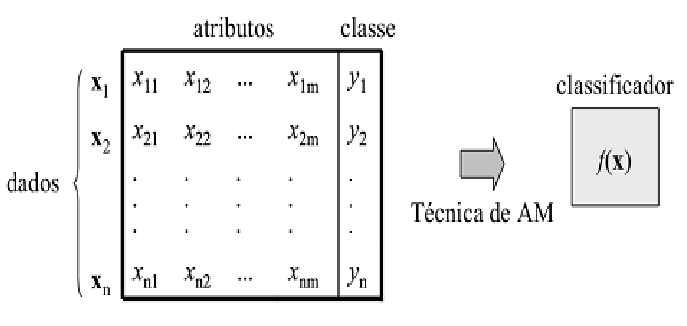
\includegraphics[scale=0.5]{./figuras/classificador_supervisionado.png}
	\caption{Classificador de aprendizagem supervisionado \cite{Lorena2007}}
	\label{fig:classificador_supervisionado}
\end{figure}


\section{Teoria do aprendizado estatístico}\label{S3}

A teoria do aprendizado estatístico (TAE) estuda as propriedades matemáticas das máquinas de aprendizagem. Estes estudos auxiliam na escolha e projeção, de uma função (ou classificador) $f$ a partir dos dados de treinamento $\tau$, tal que $f$ seja ótima. Para a escolha são utilizadas as propriedades matemáticas, que levam em conta o desempenho (p. ex. quão rápido o algoritmo converge) no conjunto de dados e a complexidade. Com isto é possível ter uma estimativa do desempenho para novos conjuntos de dados.


\begin{figure}[htb]
	\centering
	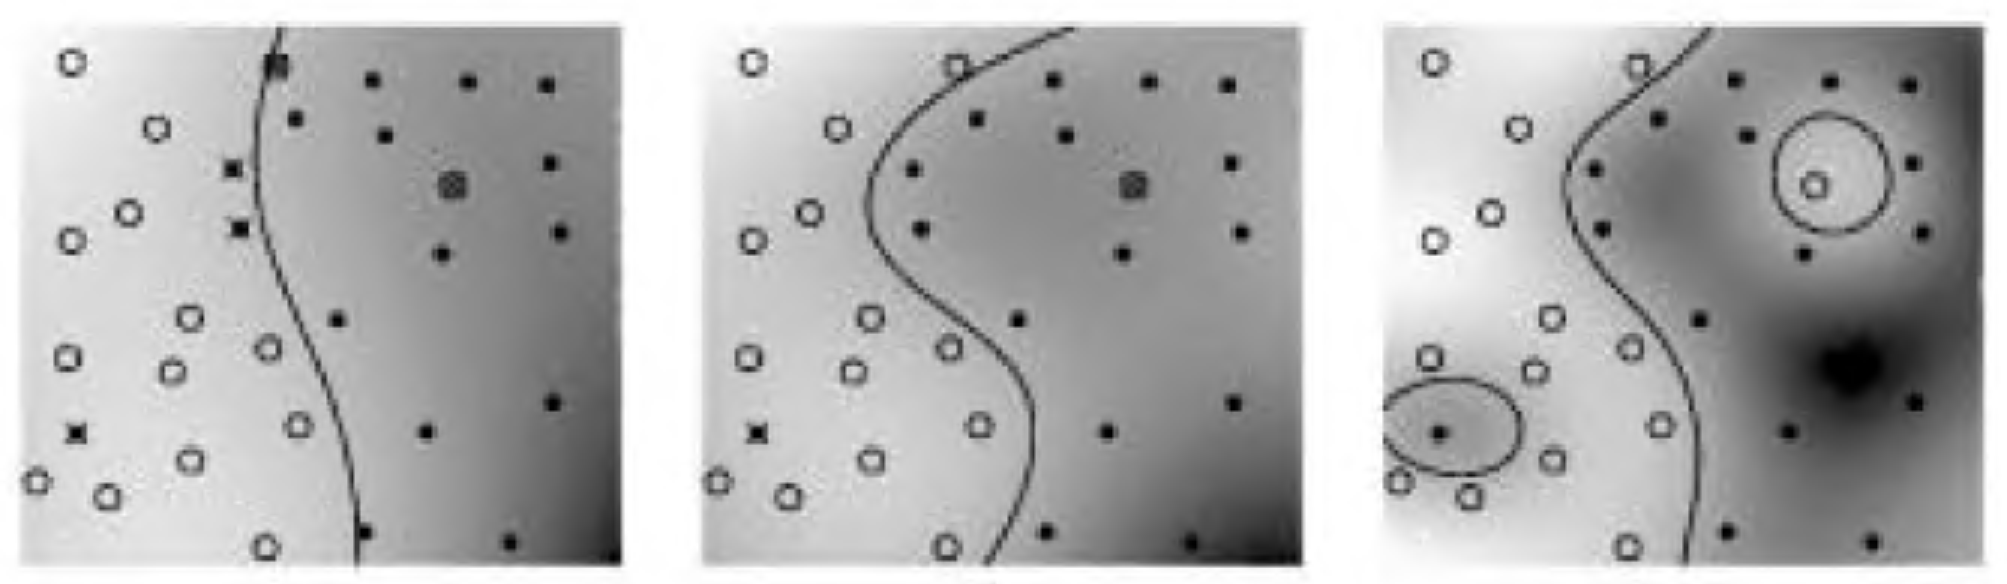
\includegraphics[scale=0.3]{./figuras/2dtoyexample.png}
	\caption{Três modelos para a classificação binaria de dados \cite{Scholkopf2002}}
	\label{fig:2dtoyexample}
\end{figure}

No exemplo dado por \cite{Scholkopf2002}, a tarefa é separar os pontos sólidos em negrito que assumem o valor 1 dos círculos que assumem o valor -1, mostrado na Figura \ref{fig:2dtoyexample}. 

No gráfico mais a direita, a função de classificação separa corretamente todos os dados, inclusive dois \textit{outliers} \footnote{Outliers são dados classificados incorretamente, tais dados invadem o espaço da classe oposta a dele.}. Porém para dados de teste é grande a probabilidade dela gerar um erro, devido a sua grande especificidade. Este tipo de caso é chamado de superajustamento do modelo aos dados de treinamento, comumente conhecido pelo termo em inglês \textit{overfitting}. Para evitar o superajustamento podemos tentar um modelo mais simples como o gráfico mais a esquerda, que tem uma função de classificação praticamente linear. Entretanto esta separação não somente desclassifica os \textit{outliers} mas também casos considerados simples. Temos assim um sub-ajustamento, porque o classificador não é capaz de ajustar até mesmo aos exemplos de treinamento. Por último, o gráfico central que tem uma complexidade intermediária e consegue classificar a maioria dos pontos corretamente.

Os dados usados na escolha do classificador são gerados de uma probabilidade de distribuição $P(x,y)$ desconhecida , tal que $f$ classifique dados que não fazem parte do conjunto de treinamento corretamente. Dados gerados dessa forma é comumente conhecidos como independente e identicamente distribuídos (\textit{iid}). 

A melhor função $f$ é a que tem o cálculo do erro esperado, ou risco, minimizado para os dados de teste. Na Equação \ref{TA:E1}, $c(f(x),y)$ é a função de ativação relacionando a previsão $f(x)$ com a saída desejada $y$. Neste caso a função de ativação é assumida como $c(f(x),y) = \frac{1}{2} \mid y - f(x) \mid$. O valor da função é definido pela Equação \ref{funcx} de acordo com \cite{Burges1998Support, Scholkopf2002}.

\begin{equation} \label{funcx}
c(f(x),y) = \left\{\begin{matrix}
0, & se\ x \text{ é classificado corretamente} \\ 
														       \\		
1, & se\ x \text{ é classificado incorretamente}
\end{matrix}\right.
\end{equation}

\begin{equation} \label{TA:E1}
R(f) = \int c(f(x),y)dP(x,y)
\end{equation}

Infelizmente o risco não pode ser minimizado diretamente, uma vez que a distribuição de probabilidade $P(x,y)$ é desconhecida. Então utilizamos o processo de minimização do risco empírico de $f$ (Equação \ref{TA:E2}), que mede o desempenho do classificador nos dados de treinamento, por meio da taxa de classificações incorretas obtidas \cite{Muller2001}.

\begin{equation} \label{TA:E2}
R_{emp}(f) = \frac{1}{n} \sum_{i=1}^n c(f(x_{i}),y_{i})
\end{equation}

É possível dar condições para a máquina de aprendizagem, a qual assegura que assintoticamente (com $n \rightarrow \infty$) o risco empírico irá convergir para o risco esperado \cite{Muller2001}. Em outras palavras, permitindo que $f$ seja escolhida a partir de um conjunto de funções $F$ é sempre possível encontrar uma $f$ com pequeno risco empírico. Entretanto para pequenas amostras pode ocorrer o superajustamento. Então um menor erro não pode ser obtido apenas minimizando o erro de treinamento. Para evitar este tipo de problema deve-se restringir a classe de funções da qual $f$ é extraída \cite{Scholkopf2002}. Para isto existem diversas abordagens, e cabe a TAE apresentar quais conjuntos tem capacidade apropriada para a quantidade de dados de treinamento para a função $f$. Esta teoria também provê limites no risco esperado de uma função de classificação, que podem ser empregados na escolha do classificador.

Um outro limite importante da TAE é o limite de risco limitado. Este relaciona o risco esperado de uma função ao seu risco empírico e a um termo de capacidade. A Equação \ref{TA:E3} apresenta o risco limitado.

\begin{equation} \label{TA:E3}
R(f)\leq R_{emp}(f)+\sqrt{\frac{h\left(ln(\frac{2n}{n})+1\right) - ln (\frac{\theta}{4})}{n}}
\end{equation}

Onde, $h$ é a dimensão Vapinik-Chevonenkis (VC) da classe de funções $F$ que $f$ pertence, o limite da Equação \ref{TA:E3} é garantido com probabilidade de $1 - \theta$, em que $\theta \in [0,1]$, $n$ representa a quantidade de dados de treinamento, e todos os elementos que estão na raiz fazem parte do termo de capacidade.

É possível fazer algumas observações no risco limitado. A primeira, é que ele é independente de $P(x,y)$, e a segunda, é que nem sempre é possível calcular o lado esquerdo da equação, porque ele depende de $P(x,y)$. Por último, se $h$ for conhecido, possibilita facilmente calcular o lado direito da equação, e escolhendo um $\theta$ pequeno, isto é escolhendo a máquina que minimiza o lado direito, estamos escolhendo a máquina com menor limite superior no risco atual \cite{Burges1998Support}.

A dimensão VC separa os dados através de uma função em um certo modo que possibilita atribuir rótulos nos dados. Como os rótulos são binários, a quantidade máxima de rótulos diferentes para $m$ dados é $2^m$. Uma função "boa"\  é capaz de realizar $2^m$ separações, neste caso é dito quebrar os $m$ pontos. A dimensão VC é definida como o maior $m$ que existe em um conjunto de $m$ pontos, que são separados pela função, e $\infty$ caso $m$ não exista \cite{Scholkopf2002}.

A Figura \ref{fig:vc-dimensionexample} mostra um exemplo de VC. Existe $2^3=8$ caminhos de separar os 3 pontos em duas classes. Os dados podem ser separados por hiperplanos e a função de classe pode quebrar 3 pontos.

\begin{figure}[htb]
	\centering
	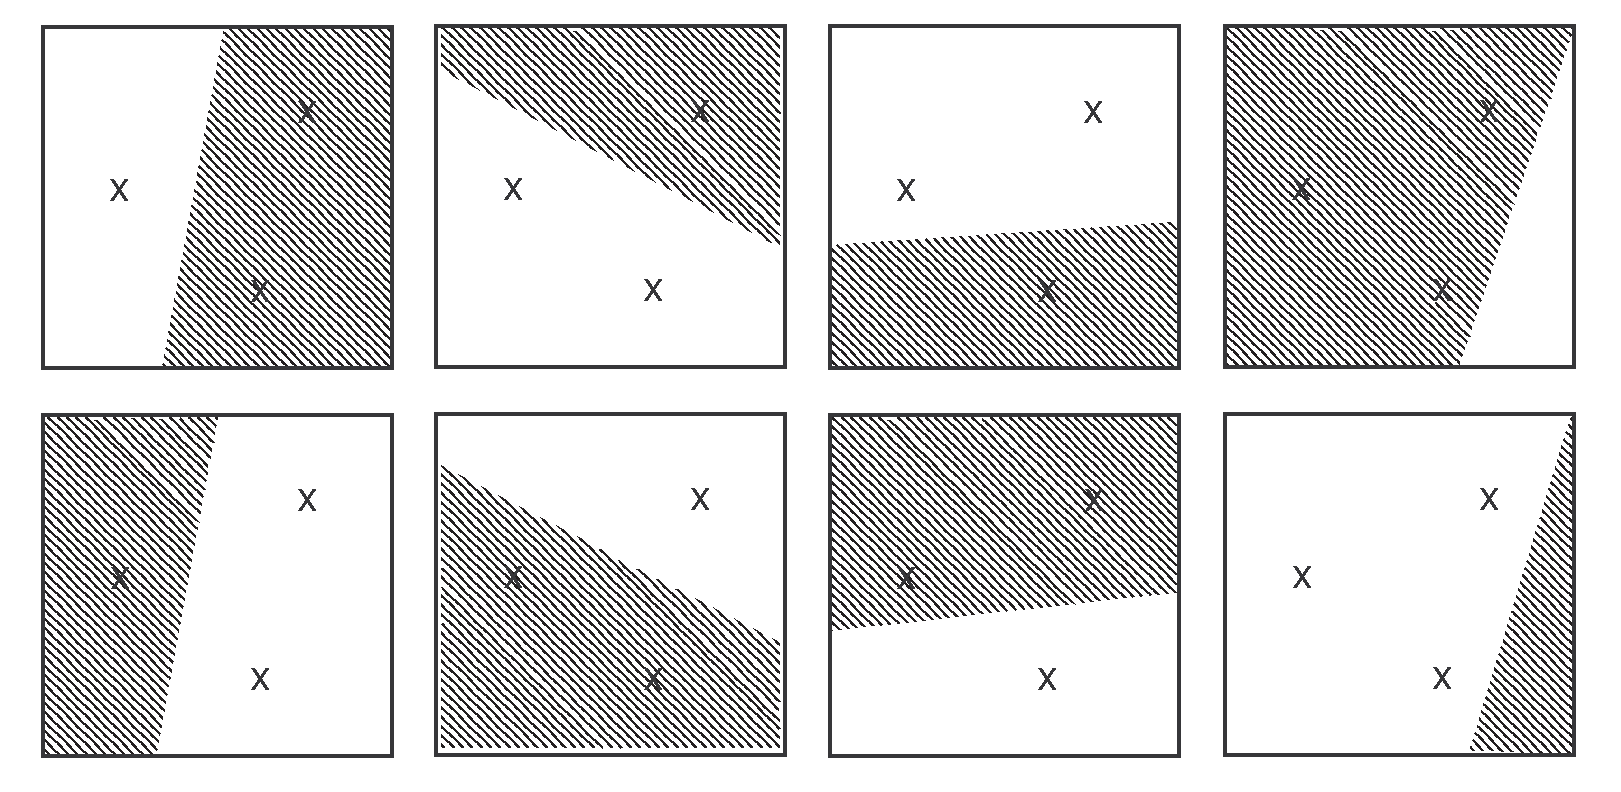
\includegraphics[scale=0.3]{./figuras/vc-dimensionexample.png}
	\caption{Exemplo de dimensão VC \cite{Scholkopf2002}}
	\label{fig:vc-dimensionexample}
\end{figure}


\section{Teoria da otimização} \label{Teot}

A teoria da otimização está relacionada no desenvolvimento da técnica do SVM, em especial em casos em que a função de custo é uma função quadrática convexa, com restrições que são lineares. Estes tipos de problemas são chamados de problemas quadráticos. O estudo destes problemas é importante, porque ele provê algoritmos e define condições para a resolução de problemas com características às da SVM \cite{Cristianini2000}. Nesta seção será apresentada de forma simplificada os problemas quadráticos \label{Teot:S1}. % falar de lagrange e dualidade

\subsection{Problema quadrático} \label{Teot:S1}

O problema quadrático na forma primal é definido da seguinte maneira:

\begin{equation} \label{Teot:E1}
\text{Minimizar}\  f(w),\ w \in \Omega
\end{equation}

\begin{equation} \label{Teot:E2}
\begin{matrix}
\text{Sujeito às restrições: } & g_{i}(w) \leq 0,\ i=1,...,k, \\ 
&    h_{i}(w) = 0,\ i=1,...,m  
\end{matrix}
\end{equation}

Onde as funções $f,\ g_{i},\ i=1,...,k, $ e $h_{i},\ i=1,...,m$ definidas no domínio $\Omega \subseteq \Re^n$, $f(w)$ é a função objetivo, $g_{i}(w)$ é a restrição de desigualdade  e $h_{i}(w)$ é a restrição de igualdade.

Uma função $f(w)$ é definida como convexa para $w \in \Re^n$ se $\forall w, u \in \Re^n$ e para qualquer $\theta \in (0,1)$, tem-se:

\begin{equation} \label{Teot:E3}
f(\theta w + (1 - \theta)u) \leq \theta f(w) + (1 - \theta)f(u).
\end{equation} 

Uma função convexa em um problema de minimização sempre possui uma solução global, o que se torna uma vantagem no tratamento do problemas quando a função é convexa \cite{Cristianini2000}. O teorema de Minimização Convexa, assegura essa propriedade onde: um conjunto convexo $D \subset \Re^n$ e $f:D \rightarrow \Re$ uma função convexa em $D$. Então todo o minimizador local da função $f(x)$ em $x \in D$ é global \cite{Ales2008}.

\subsection{Teoria do Lagrangeano}\label{Teot:S2}

Esta teoria foi desenvolvida por Lagrange em 1797, que generalizava um resultado de Fermat de 1629, posteriormente em 1951 foi estendida por Kuhn e Tucker. A junção destes avanços provê eficientes soluções para a tarefa de otimização de SVMs.

\textbf{Teorema de Fermat} A condição necessária para que $w^*$ seja mínimo de $f(w), f \in C^1$, é:

\begin{equation} \label{Teot:E4}
\frac{\partial f(w^*)}{\partial w} = 0
\end{equation}

Desde que $f$ seja um função convexa, essa condição é o suficiente. Em resumo, se $f \in C^1$, basta encontrar o ponto com a derivada primeira igual à zero, que será encontrado o mínimo da função.

Precisamente, um Lagrangiano é definido como a função objetivo somado a combinação linear das restrições, onde os coeficientes de combinação são chamados de multiplicadores de Lagrange \cite{Cristianini2000}. 

Dado um problema de otimização com função objetivo $f(w)$, e restrições de igualdade $h_{i}(w) = 0, i=1,...,m$, a função Lagrangiana é definida como:

\begin{equation}\label{Teot:E5}
L(w,\alpha) = f(w) + \sum_{i=1}^m \alpha_{i} h_{i}(w)
\end{equation}

Onde os coeficientes $\alpha_{i}$ são os multiplicadores de Lagrange.

\textbf{Teorema de Lagrange} Uma condição necessária para um ponto $w^*$ ser mínimo da função $f(w)$ sujeito a $h_{i}(w) = 0, i-1,...,m$ com $f,h_{i} \in C^1$, é:

\begin{equation} \label{Teot:E6}
\begin{matrix}
\frac{\partial L(w^*, \alpha^*)}{\partial w}  = 0 \\ \\
\frac{\partial L(w^*, \alpha^*)}{\partial \alpha} = 0
\end{matrix}
\end{equation}

para algum valor de $\alpha^*$. Isto prova que $L(w,\alpha^*)$ é uma função convexa de $w$.

A definição generalizada da função Lagrangeana, onde o problema de otimização contém as restrições de igualdade e desigualdade é: dados o problema de otimização \ref{Teot:E2} e o domínio $\Omega \subseteq \Re^n$ defini-se a função Lagrangeana Generalizada com mostrado na Equação \ref{Teot:E7}.

\begin{equation}\label{Teot:E7}
L(w,\alpha,\beta) = f(w) + \sum_{i=1}^k \beta_{i}g_{i}(w)+\sum_{i=1}^m \alpha_{i}h_{i}(w) = f(w)+\beta ' g(w)+\alpha ' h(w)
\end{equation}

O próximo passo é definir Lagrange na forma de problema dual. O problema dual é associado ao problema original (primal) facilitando a resolução do problema.

O problema dual Langrangeano pode ser definido como: dado um problema na forma primal \ref{Teot:E2}, com $\Omega \in \Re^n$, o problema dual é dado pela Equação \ref{Teot:E8}.

\begin{equation} \label{Teot:E8}
\begin{matrix}
\text{Maximizar} & \theta(\alpha,\beta) \\ 
\text{Sujeito as restrições}&    \alpha \geq 0
\end{matrix}
\end{equation}

onde: $\theta(\alpha,\beta) = inf_{w \in \Omega}L(w,\alpha,\beta)$

Uma importante definição que surge é o \textit{Gap} Dual. \textit{Gap} é a diferença entre os valores da função objetivo do modelo primal e do modelo dual \cite{Cristianini2000}. O \textit{gap} está relacionado com a solução ótima encontrada quando o valor da função objetivo primal $w$ é igual à função objetivo dual $\theta$, quanto mais próximo de zero estiver o \textit{gap} dual, mais próximo está da solução ótima do problema.

O teorema forte da dualidade afirma o que foi mencionado no parágrafo anterior, onde dado um problema de otimização \ref{Teot:E2}, com $\Omega \in \Re^n$, onde $g_{i},h_{i}$ são funções afins, o \textit{gap} dual é zero. Isto garante que os problemas dual e primal tenham o mesmo valor para problemas de otimização \cite{Cristianini2000}.

A solução ótima para um problema otimização generalizado, é condicionada ao teorema de Kuhn-Tucker. Onde, dado um problema de otimização \ref{Teot:E2}, com $\Omega \in \Re^n$, com $f \in C^1$ e $g_{i},h_{i}$ com funções afins, as condições necessárias e suficientes para que $w^*$ seja ótimo são a existência de $\alpha^*,\beta^*$, tais que:

\begin{equation}
\begin{matrix}
\frac{\partial L(w^*,\alpha^*,\beta^*)}{\partial w} = 0 \\ 
\frac{\partial L(w^*,\alpha^*,\beta^*)}{\partial \alpha} = 0 \\ 
\beta_{i}g_{i}(w^*) = 0 \\
g_{i}(w^*) \leq 0 \\
\beta^* \geq 0, i=1,...,k.
\end{matrix}
\end{equation}

%O resulta acima mostra que a definição de Multiplicador de Lagrange é uma extensão da noção do multiplicador na condição  de Karush-Kuhn-Tucker \cite{Cristianini2000}.

Toda a teoria estudada é fundamental para o entendimento teórico da SVM, uma vez que a SVM envolve a minimização de um problema quadrático convexo.

\section{SVMs lineares}\label{cap:svm:svm-l}

A teoria da SVM está fortemente ligada com a teoria da dimensão VC, uma vez que, na SVM é feito uma separação dos dados através de um hiperplano. A dimensão VC pode ser limitada pela margem: rígida ou suave. A diferença entre os dois grupos é que os classificadores SVM de margem rígida não permitem ruídos e \textit{outliers} nos dados, já a margem suave é uma extensão mais relaxada da SVM com margem rígida, permitindo tais tipos de dados. Primeiramente será abordado a SVM com margem rígida, que é um caso mais simples com fins didáticos. Para problemas práticos a SVM com margens suave é mais apropriada, esta será abordada na sequência.

\subsection{SVM com margem rígida} \label{svmL:S1}

Assume-se um conjunto de treinamento de dados $T$ com $n$ dados formado pelo par de dados $(x_{i},y_{i})$ onde $x_{i} (i = 1,....,n ), x_{i} \in R^{d}, d = 1,2,...,d $  são os dados de treinamento e $y_{i} (i = 1,....,n), y_{i} \in {-1,+1}$ são os respectivos rótulos de $x_{i}$. Os rótulos $y_{i}$ assumem dois possíveis valores $+1$ para dados da classe 1 e $-1$ para dados da classe 2. Se estes dados são linearmente separáveis, existe uma superfície de decisão que separa os dados positivos (+1) dos negativos (-1). A equação da superfície de decisão na forma de um hiperplano separador é apresentada na Equação \ref{svm:hp-sep}, onde $w\cdot x$ é o produto escalar entre os vetores $w$ e $x$, $w$ é um vetor de pesos ajustável, e $w \in R^{d}$, portanto $w$ também faz parte do conjunto de entradas (ou dados de treinamento), $b \in R$ é um bias. Os pontos $x$ que se encontram no hiperplano satisfazem $w\cdot x + b = 0$, onde $w$ é perpendicular ao hiperplano e $ \frac{b}{\parallel w \parallel}$ é a distância perpendicular do hiperplano até a origem \cite{Burges1998Support}.
%A menor distância distancia do dado mais próximo do hiperplano separador é chamado de $d_{+}$ para dados positivos ou $d_{-}$ para dados negativos. Uma margem de um hiperplano separador é a soma das distâncias positivas e negativas($d_{+}+d_{-}$) 

\begin{equation} \label{svm:hp-sep}
	f(x) = w\cdot x + b = 0
\end{equation}

Multiplicando $w$ e $b$ pela mesma constante é possível obter infinitos hiperplanos equivalentes. Um hiperplano é definido na forma canonical, se $w$ e $b$ são escalados de tal forma que os dados mais próximos do hiperplano $w\cdot x + b = 0$ satisfaça a Equação \ref{svm:E2} \cite{Scholkopf2002}:

\begin{equation} \label{svm:E2}
	\mid w\cdot x_{i} + b\mid = 1
\end{equation}
 
Essa forma implica na inequação \ref{svm:E3}.
\begin{equation} \label{svm:E3}
\left\{\begin{matrix}
w \cdot x_{i}+b \geq + 1 & para & y_{i} = +1 \\ 
w \cdot x_{i}+b \leq + 1 & para & y_{i} = -1
\end{matrix}\right.
\end{equation}

Que pode ser combinadas em um conjunto de inequações:

\begin{equation}\label{svm:E4}
y_{i}(x_{i} \cdot w+b) - 1 \geq 0 \ \ \    \forall i
\end{equation}

Se os dados são linearmente separados eles estão restritos a condição da Equação \ref{svm:E4}. É possível definir um hiperplano canônico $H_{1}:w \cdot x + 1 = +1$ para os pontos dos dados positivos e $H_{2}:w \cdot x + 1 = -1$ para os pontos dos dados negativos. A projeção de $x_{1}$ - $x_{2}$ no vetor $w$, nos dá a margem, onde $x_{1}$ e $x_{2}$ são pontos próximos ao hiperplano separador mas em lados opostos \cite{Campbell2001}. 

\begin{equation}\label{svm:E5}
(x_{1} - x_{2})\left(\frac{w}{\parallel w \parallel} \cdot \frac{(x_{1} - x_{2})}{\parallel x_{1} - x_{2} \parallel} \right)
\end{equation}

Temos as equações $w \cdot x_{1} + b = +1$ e $w \cdot x_{1} + b = -1$, fazendo a diferença entre elas obtemos a Equação \ref{svm:E6} \cite{Hearst1998}. 

\begin{equation} \label{svm:E6}
w \cdot (x_{1} - x_{2}) = 2
\end{equation}

Substituindo \ref{svm:E6} em \ref{svm:E5} temos:

\begin{equation}\label{svm:E7}
\frac{2(x_{1}-x_{2})}{\parallel w \parallel \parallel x_{1}-x_{2} \parallel}
\end{equation}

Tomando a norma da Equação \ref{svm:E7}, temos o comprimento do vetor projetado:

\begin{equation} \label{svm:E8}
\frac{2}{\parallel w \parallel}
\end{equation}

Que é a distância $d$, entre os hiperplanos $H_{1}$ e $H_{2}$, que são paralelos ao hiperplano separador, a Figura \ref{fig:margem_svm} mostra o hiperplano separador e os hiperplanos $H_{1}$ e $H_{2}$, nota-se que eles são paralelos e que nenhum dado de treinamento fica entre eles, os dados que tocam os hiperplanos $H_{1}$ e $H_{2}$, são chamados de vetores de suporte(p. ex. $x_{1}$ e $x_{2}$).

\begin{figure}[htb]
	\centering
	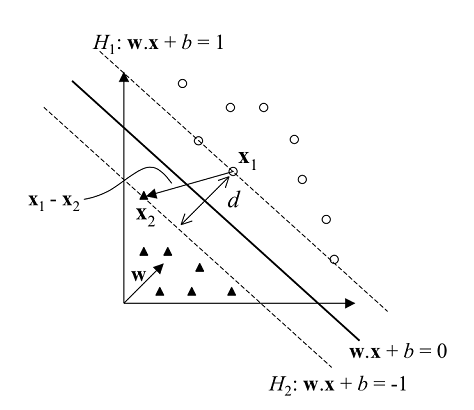
\includegraphics[scale=0.5]{./figuras/margem_svm.png}
	\caption{Hiperplano separador representado pela linha no meio e hiperplanos de apoio $H_{1}$ e $H_{2}$ representado pelas retas pontinhadas nas extremidades, assim com os vetores de suporte como $x_{1}$ e $x_{2}$ e a distância $d$ (Adaptado de \cite{Lorena2007}}
	\label{fig:margem_svm}
\end{figure}

Para maximizar a distância $d$, onde procura-se encontrar a distância que melhor separa os dados, podemos recorrer ao seguinte problema de otimização:

\begin{equation} \label{svm:E9}
\text{Minimizar}_{w,b}\  \frac{1}{2}\parallel w \parallel^{2}
\end{equation}

\begin{equation} \label{svm:E10}
\text{Sujeito às restrições: } y_{i}(w \cdot x_{i} + b) - 1 \geq 0, \ \ \forall i=1,...,n
\end{equation}

Note que a restrição impede que haja dados de treinamento entre as margens de separação das classes. Por isso o nome de SVM de margens rígidas.

O problema obtido é do tipo quadrático, para a resolução desse problema existem vários métodos que serão visto na Seção \ref{spq}. Para a resolução de problemas dessa categoria é necessário a substituição da formulação do problema para uma formulação Lagrangiana. Isto é feito porque a restrição \ref{svm:E10} será substituída por restrições na forma de multiplicadores de Lagrange, que trazem facilidades na resolução. Outro motivo, é que os dados de treinamento irão aparecer somente na forma de produto interno entre os dados, que irá ajudar no procedimento de generalização no caso não-linear(\ref{cap:svm:svm-nl}) \cite{Burges1998Support}. Transformando as Equações \ref{svm:E9} e \ref{svm:E10}, em uma função Lagrangiana obtemos:

\begin{equation} \label{svm:E11}
L(w,b,\alpha) = \frac{1}{2}\parallel w \parallel^2 - \sum_{i}^{n} \alpha_{i}(y_{i}(w \cdot x_{i} + b) - 1)
\end{equation}

Para minimizar a função Lagrangiana, é necessário maximizar as variáveis $\alpha_{i}$ e minimizar $w$ e $b$. Calculando o gradiente de $L$ em relação a $w$ e $b$ nos da as seguintes condições \cite{Burges1998Support}:

\begin{equation}\label{svm:E12}
w = \sum_{i = 1}^{n} \alpha_{i}y_{i}x_{i}
\end{equation}

\begin{equation}\label{svm:E13}
\sum_{i = 1}^{n} \alpha_{i}y_{i} = 0
\end{equation}

Substituindo as Equações \ref{svm:E12} e \ref{svm:E13} na Equação \ref{svm:E11} obtemos:

\begin{equation}\label{svm:E14}
\text{Maximizar}_{\alpha} \sum_{i = 1}^{n} \alpha_{i} - \frac{1}{2} \sum_{i,j = 1}^{n} \alpha_{i}\alpha_{j}y_{i}y_{j}(x_{i} \cdot x_{j})
\end{equation}

\begin{equation} \label{svm:E15}
\text{Sujeito às restrições:} 
\left\{\begin{matrix}
\alpha \geq 0, \  \forall i = 1,...,n \\ 
\sum_{i = 1}^{n} \alpha_{i}y_{i} = 0  &
\end{matrix}\right.
\end{equation}

Este tipo de formulação é conhecido como a forma dual, e a anterior (sem multiplicadores de Lagrange) como forma primal. 

Na solução dual para cada dado de treinamento temos um $\alpha_{i}$, e todos os dados onde $\alpha_{i} > 0$, são chamados de vetores de suporte, e estão localizados em um dos hiperplanos $H_{1}$ ou $H_{2}$. Os dados cujo o $\alpha_{i} = 0$, estão no mesmo lado de $H_{1}$ ou $H_{2}$, de tal forma que não viole a restrição imposta na Equação \ref{svm:E10}. Esses dados não participam do cálculo de $w$ (Equação\ref{svm:E12}). Para encontrar o valor de $b$, são feitos cálculos a partir do vetores de suporte (VT) conforme é mostrado na Equação \ref{svm:E16}.

\begin{equation} \label{svm:E16}
b = \frac{1}{n_{VT}} \sum_{x_{j} \in VT} \left(\frac{1}{y_{j}} - \sum_{x_{j} \in VT} \alpha_{i}y_{i}x_{i} \cdot x_{j} \right)
\end{equation}
onde $n_{VT}$ é o número de vetores de suporte.

Assim chegamos a função do classificador linear (Equação \ref{svm:E17}), está função representa o hiperplano que separa os dados com a margem, considerando aqueles com maior capacidade de generalização.

\begin{equation} \label{svm:E17}
f(x) = \left(\sum_{x_{i} \in VT} y_{i}\alpha_{i}x_{i} \cdot x + b \right)
\end{equation}

\subsection{SVM com margem suave}
Nas SVMs com a margem rígida é assumido que os dados são totalmente heterogêneos, com solução só para casos sem a presença de ruídos ou \textit{outliers}. Entretanto na prática é comum que os dados contenham ruídos e \textit{outliers}. Nesta seção veremos como contornar este obstaculo com a introdução das SVMs de margem suave. Isto é feito através da generalização do caso com margens rígidas, introduzindo um variável de folga $\xi_{i}, i= 1,...,l$, nas restrições impostas ao problema de otimização primal, que se tornam  \cite{Scholkopf2002}: 

\begin{equation} \label{svm:E18}
y_{i}(w \cdot x_{i} + b) \geq 1 - \xi_{i}, \  \xi_{i} \geq 0, \forall i =1,...,n
\end{equation}

Com a aplicação do $\xi_{i}$, as margens do classificador ficara suavizada, permitindo que dados permaneçam entre os hiperplanos $H_{1}$ e $H_{2}$, assim como erros de classificação.

Para que ocorra um erro é necessário que o erro exceda um limite. Este limite é a soma dos $\sum_{i} \xi_{i}$ que é um limite superior do número de erros de treinamento \cite{Burges1998Support}. Devemos modificar a função objetivo da Equação \ref{svm:E9} para conter o custo extra para erros, que fica:

\begin{equation}\label{svm:E19}
\text{Minimizar}_{w,b,\xi} \frac{1}{2}\parallel w \parallel^{2} + C \left( \sum_{i=1}^n \xi_{i}\right)
\end{equation}

A constante $C$ é um parâmetro definido pelo usuário e ela atua como um termo de regularização da complexidade do modelo em relação a margem de erros, um valor alto de $C$ significa uma alta penalidade para erros \cite{passerini04kernelmethods}

O problema de otimização gerado novamente é quadrático semelhante ao de margens rígidas, mas com as restrições da Equação \ref{svm:E18}, com os multiplicadores de Lagrange temos o seguinte problema dual:

\begin{equation}\label{svm:E20}
\text{Maximizar}_{\alpha} \sum_{i = 1}^{n} \alpha_{i} - \frac{1}{2} \sum_{i,j = 1}^{n} \alpha_{i}\alpha_{j}y_{i}y_{j}(x_{i} \cdot x_{j})
\end{equation}

\begin{equation} \label{svm:E21}
\text{Sujeito as restrições:} 
\left\{\begin{matrix}
0 \leq \alpha \leq C, \  \forall i = 1,...,n \\ 
\sum_{i = 1}^{n} \alpha_{i}y_{i} = 0  &
\end{matrix}\right.
\end{equation}

A única diferença em relação ao caso anterior é que o $\alpha_{i}$ tem um limite superior de $C$. Para uma solução ótima
do problema dual, encontramos o valor das variáveis $\xi_{i}$ pela seguinte equação:

\begin{equation}\label{svm:E22}
\xi_{i} = max \left\lbrace 0,1 - y_{i} \sum_{j=1}^{n}y_{j}\alpha_{j}x_{j} \cdot x_{i} + b \right\rbrace
\end{equation}

Para encontrar $b$ como no caso rígido ele provém de $\alpha$ e de condições KKT( Karush-Kuhn-Tucker) representadas nas Equações \ref{svm:E23} e \ref{svm:E24} \cite{Scholkopf2002}.

\begin{equation} \label{svm:E23}
\alpha_{i}(y_{i}(w \cdot x_{i} + b) - 1 + \xi_{i}) = 0
\end{equation}

\begin{equation} \label{svm:E24}
(C - \alpha_{i})\xi_{i} = 0
\end{equation}

Pelas condições de KKT das Equações \ref{svm:E23} e \ref{svm:E24}, podemos definir os vetores de suporte que diferente do caso rígido pode assumir três tipos distintos \cite{Scholkopf2002}:
\begin{itemize}
\item $\alpha_{i} = 0$ e $\xi_{i} = 0$. Então o dado $x_{i}$ é corretamente classificado e encontra-se fora das margens.
\item $0 < \alpha_{i} < C$ e $\xi_{i} = 0$. Então o dado $x_{i}$ é um vetor de suporte que encontra-se entre as margens, também denominado de livres.
\item $\alpha = C$. Então temos três casos: o dado $x_{i}$ é um erro se e $\xi_{i} > 1$; $x_{i}$ é classificado corretamente mas entre as margens,se $0 < \xi_{i} \leq 1$; ou $x_{i}$ fica sobre as margens, se $\xi_{i} = 0$.
\end{itemize}

\begin{figure}[htb]
	\centering
	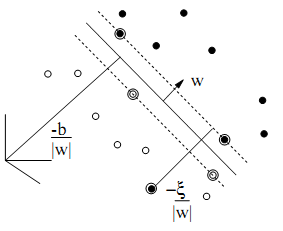
\includegraphics[scale=0.9]{./figuras/margem_svm_suave.png}
	\caption{Exemplo de classificador SVM com margens suaves (Adaptado de \cite{Burges1998Support}}
	\label{fig:margem_svm_suave}
\end{figure}

Na Figura \ref{fig:margem_svm_suave} os dados circulados na linha tracejada são os vetores de suporte livres. O dado de cor preta que está do outro lado do hiperplano é considerado um erro. 

\section{SVMs não-linear}\label{cap:svm:svm-nl}

As SVMs lineares descritas anteriormente são eficazes na classificação de dados que podem ser separados linearmente por um hiperplano. Porém para os dados de treinamento que não são separáveis linearmente, as SVMs não conseguem obter resultados satisfatórios. Para contornar esse problema será introduzido as SVMs não-linear. Para o caso não-linear é necessário a transformação dos dados de seu espaço original $x$ para um novo espaço de maior dimensão $\Phi(x)$ onde é possível separar os dados linearmente. Então é aplicado a metodologia apresentada para o caso linear, para encontrar o hiperplano separador nos dados transformados classificando-os corretamente \cite{Steinbach2005}. As Figuras \ref{fig:1d-to-2d-svm} e \ref{fig:2d-to-3d}, são dois exemplos de dados que em seus espaços originais não é possível separa-los com um hiperplano mas quando transformamos o espaço para outra dimensão, é possível fazer a separação dos dados.

\begin{figure}[htb]
	\centering
	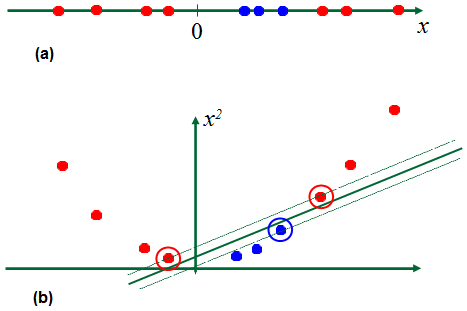
\includegraphics[scale=0.5]{./figuras/1d-to-2d-svm.png}
	\caption{(a) Conjunto de dados que não podem ser separados no espaço original; (b) Transformação do espaço para que seja possível a separação dos dados}
	\label{fig:1d-to-2d-svm}
\end{figure}

\begin{figure}[htb]
	\centering
	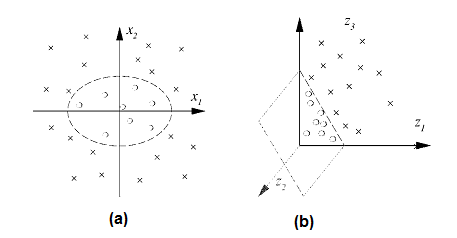
\includegraphics[scale=0.8]{./figuras/2d-to-3d.png}
	\caption{(a) Conjunto dados não linear; (b) Separação dos dados em (a) com a transformação do espaço (Adaptado de \cite{Muller2001})}
	\label{fig:2d-to-3d}
\end{figure}

No processo de transformação dos dados $\Phi: \Re^{d} \rightarrow \aleph$ é um mapeamento, onde $\Re^{d}$ é o espaço de entradas e $\aleph$ é o novo espaço com dimensão maior, também conhecido com espaço de características. Nosso objetivo é escolher corretamente $\Phi$, para que o conjunto de treinamento seja mapeado em $\aleph$ onde a fronteira de decisão é linear.

\cite{Muller2001} apresenta um exemplo simples desse mapeamento, que é a transformação feita na Figura \ref{fig:2d-to-3d}, onde os dados em $\Re^2$ são mapeados para a $\Re^3$. Para fazer o mapeamento $\Phi:\Re^2 \rightarrow \Re^3$ é utilizado a Equação \ref{svm:E25}, aplicando a equação o conjunto de dados em $\Re^2$ transforma-se em dados linearmente separáveis em $\Re^3$. Em $\Re^3$ é possível encontrar um hiperplano que separa os dados (Equação \ref{svm:26}). Embora a equação do hiperplano seja linear em $\Re^3$ ela não é linear em $\Re^2$.

\begin{equation}\label{svm:E25}
\Phi(x) = \Phi(x_{1},x_{2}) = \left(x_{1}^2,\sqrt{2x_{1}}x_{2},x_{2}^2\right)
\end{equation}

\begin{equation} \label{svm:E26}
f(x) = w \cdot \Phi(x) + b = w_{1}x_{1}^2 + w_{2} \sqrt{2x_{1}}x_{2} + w_{3}x_{2}^2 + b = 0
\end{equation}

A separação dos dados na nova dimensão é feita com a SVM de margens suáveis, para permitir ruídos e \textit{outliers}. Coma a adição do mapeamento de dados $\Phi$ a função de otimização da Equação \ref{svm:E20} fica conforme representado na Equação \ref{svm:E27}. As restrições são as mesmas da SVM linear de margens suáveis (Equação \ref{svm:E21}). E a função de decisão será na forma apresentada na Equação

\begin{equation} \label{svm:E27}
\begin{matrix}
\text{Maximizar}_{\alpha} \sum_{i = 1}^{n} \alpha_{i} - \frac{1}{2} \sum_{i,j = 1}^{n} \alpha_{i}\alpha_{j}y_{i}y_{j}(\Phi(x_{i}) \cdot \Phi(x_{j})) \\ 
0 \leq \alpha \leq C,\  \forall i = 1,...,n \\
\sum_{i = 1}^{n} \alpha_{i}y_{i} = 0
\end{matrix}.
\end{equation}



\begin{equation} \label{svm:E28}
f(x) = \sum_{x_{i} \in SV}\alpha_{i}y_{i}\Phi(x_{i}) \cdot \Phi(x) + b
\end{equation}

Nota-se pela Equação \ref{svm:E28} que os dados aparecem na forma de produtos interno, $\Phi(x_{i} \cdot \Phi_{j})$, e que a única informação necessária para o mapeamento é como realizar o produto interno. Este tipo calculo é muito custoso \cite{Scholkopf2002}, mas ele pode ser reduzido para uma função \textit{Kernel} $K$ tal que:

\begin{equation} \label{svm:E29}
K(x_{i},x_{j}) = \Phi(x_{i}) \cdot \Phi(x_{j}))
\end{equation} 
 
Assim só usamos $k$ no algoritmo de treinamento, sem a necessidade de explicitar ou saber o que é $\Phi$ \cite{Burges1998Support}.

As funções kernel utilizadas nas SVMs seguem as condições estabelecidas pelo teorema de Mercer \cite{Burges1998Support}. É utilizado este teorema para que seja garantida a convexidade do problema de otimização (Equação \ref{svm:E27}) e para que os mapeamentos representados pelo kernel possibilite o cálculo de produtos escalares (Equação \ref{svm:E29}).

Não existe uma função \textit{kernel} melhor do as outras, o desempenho depende do tipo de dados de cada aplicação. A seguir serão apresentados as funções \textit{kernel} mais comum, que são:
\begin{itemize}
\item Produto interno:
\begin{equation}
K(x_{i},x_{j}) = x_{i}^T \cdot x_{j}
\end{equation}

\item Polinomial Homogêneo:
\begin{equation}
K(x_{i},x_{j}) = (x_{i}^T \cdot x_{j})^p
\end{equation}
onde:
$p$ é o grau do polinômio

\item Polinomial Não Homogêneo:
\begin{equation}
K(x_{i},x_{j}) = (x_{i}^T + c)^p
\end{equation}
onde:
$p$ é o grau do polinômio
$c$ é uma constante

\item Sigmoidal:
\begin{equation}
K(x_{i},x_{j}) = tanh(\kappa x_{i} \cdot x_{j} + c)
\end{equation}
onde:
$\kappa$ é um coeficiente
$c$ é uma constante

\item Gaussiano:
\begin{equation}
K(x_{i},x_{j}) = e^{\frac{\mid x_{i} - x_{j} \mid}{2\sigma^2} }
\end{equation}
onde:
$\sigma$ é um parâmetro
\end{itemize}

\section{Soluções da programação quadrática do SVM}\label{spq}

A modelagem do SVM envolve o problema de programação quadrática apresentado na Seção \ref{Teot}. Foram propostos vários métodos para sua resolução. Entretanto devido ao grande tamanho das entradas, a forma quadrática (Equação \ref{svm:E27}) que aparece não pode ser resolvida facilmente pelas técnicas padrão de programação quadrática. Está seção revisará os principais métodos. Iniciaremos com o método Chunking (Subseção \ref{spqS1}), na sequência o método de Decomposição (Subseção \ref{spqS2}), e finalmente (Subseção \ref{spqS3}) o \textit{Sequential Minimal Optimization} (SMO), neste será dado maior atenção, por ele ser de fácil implementação, de baixa complexidade e obter resultados satisfatórios e muitas vezes superiores que os demais métodos.

\subsection{Chunking} \label{spqS1}

Este método trabalha apenas com uma parte dos dados e utilizar somente vetores de suporte para encontrar a solução. Ele começa com uma parte arbitrária dos dados chamada '\textit{chunk}', então treina a SVM usando um otimizador quadrático qualquer. Do subconjunto treinado é mantido apenas os vetores de suporte, os demais são todos descartados, e é testado a hipótese encontrada com os vetores de suporte no restante dos dados. Os $M$ piores dados de treinamento, que violam as condições de KKT (onde $M$ é um parâmetro), são adicionados no conjunto de vetores de suporte encontrados no passo anterior para formar um novo '\textit{chunk}'. Se existe um numero menor que $M$ de exemplos que violam KKT, todos os dados que violam são adicionados ao conjunto. As iterações continuam até um critério de parada ser atingido, este critério, por exemplo, pode ser um limite no número de iterações ou até que todos os dados forem processados. Este método possui algumas falhas. A primeira é que o conjunto de vetores de suporte são armazenados na memória se esse conjunto for muito grande poderá ocorrer problemas por falta de memória. Outro problema que também envolve o tamanho do conjunto de vetores, é a falha de alguns otimizadores quadrático, devido a o conjunto ser extenso \cite{Cristianini2000,Platt1999}.

\subsection{Decomposição} \label{spqS2}

Semelhante ao método de \textit{Chunking}, o método de decomposição também reparte o problema quadrático em vários subproblemas. A principal diferença entre eles, é que no método de decomposição o subconjunto tem um número fixado de elementos. Então para cada item adicionado ao conjunto outro tem que ser removido. Neste algoritmo não será identificado todos os vetores de suporte, mas sim aqueles que otimizam o problema globalmente. Para isto os pontos incluídos no conjunto de trabalho são os que violam as condição KKT. Assim com no anterior a computação do problema quadrático é feita externamente.

\subsection{Sequential Minimal Optimization} \label{spqS3}

O \textit{Sequential Minimal Optimization} (SMO) é um algoritmo que resolve o problema quadrático de forma eficiente, rápida e sem muitos gastos de memória, uma vez que não é necessário guardar um conjunto de vetores de suporte na memória. Este algoritmo foi introduzido por \cite{Platt1999}. Ele tem algumas semelhanças com os algoritmos descritos nas seções anteriores, por exemplo ele também trabalha com subproblemas, mas contendo apenas dois pontos em cada iteração. O ponto chave deste algoritmo que o faz obter resultados melhores que os demais é que quando o conjunto de trabalho tem apenas dois elementos é possível resolver o problema analiticamente, eliminando a necessidade de usar um otimizador quadráticos como parte do algoritmo (pacote de terceiros). 

Destacam-se três componentes no SMO: o método analítico para resolver os dois pontos, uma heurística para escolher qual ponto otimizar, e um método para calcular o bias $b$. Estes três componeste serão discutidos a seguir.

\subsubsection{Solução analítica para dois pontos}

Vamos assumir que os pontos escolhidos para a solução analítica são $\alpha_{1} \ e \  \alpha_{2}$, que são multiplicadores. Primeiramente o SMO computa as restrições nos multiplicadores e então resolve para a restrição máxima. As restrições são representadas na Figura \ref{fig:smo-restric}.

\begin{figure}[htb]
	\centering
	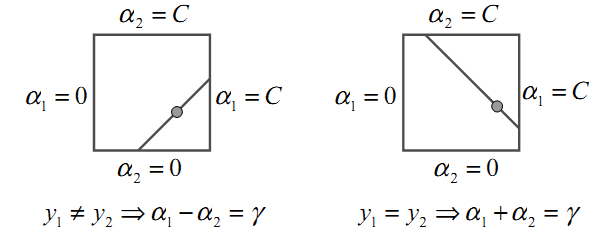
\includegraphics[scale=0.7]{./figuras/smo-restric.png}
	\caption{Restrições nos dois multiplicadores}
	\label{fig:smo-restric}
\end{figure}

O limite de restrição em \ref{svm:E27} ($0 \leq \alpha_{i} \leq C$) faz com que os multiplicadores de Lagrange repouse em uma caixa, enquanto que a equação linear de \ref{svm:E27} ($\sum_{i}^l y_{i}\alpha_{i} = 0$), faz os multiplicadores repousarem em uma linha diagonal. A restrição máxima da função objetivo irá repousar em uma reta diagonal \cite{Platt1999}. O problema de uma dimensão resultante da restrição da função objetivo pode ser solucionado analiticamente.

O algoritmo primeiramente computa $\alpha_{2}^{novo}$ e sucessivamente usa-o para obter $\alpha_{1}^{novo}$. A restrição $0 \leq \alpha_{i} \leq C$ juntamente com a restrição linear, prove uma restrição mais rígida nos possíveis valores para $\alpha_{2}^{novo}$.

\begin{equation}\label{spq:E1}
L \leq \alpha_{2}^{novo} \leq H
\end{equation}
onde:
\begin{equation}\label{spq:E2}
L = max(0, \alpha_{2}^{antigo} - \alpha_{1}^{antigo}),\ \ \ \ H = min(C, C - \alpha_{1}^{antigo} + \alpha_{2}^{antigo}),
\end{equation}
se $y_{1} \neq y_{2}$, e

\begin{equation}\label{spq:E3}
L = max(0, \alpha_{1}^{antigo} + \alpha_{2}^{antigo} - C),\ \ \ \ H = min(C, \alpha_{1}^{antigo} + \alpha_{2}^{antigo}),
\end{equation}
se $y_{1} = y_{2}$.

Para encontrar o máximo da função objetivo \ref{svm:E27}, utilizaremos o erro definido na Equação \ref{spq:E4} , que é a diferença entre a função de saída e do valor desejado.

\begin{equation}\label{spq:E4}
E_{i} = f(x) - y_{i} = \left(\sum_{j=1}^{j} \alpha_{j}y_{j}K(x_{j},x_{i}) + b \right) - y_{i},i=1,2
\end{equation}

Também é necessário um valor adicional que é a derivada da função objetivo ao longo da linha diagonal, que pode ser expressada por $k$, definido por:

\begin{equation}\label{spq:E5}
k = K(x_{1},x_{1})+K(x_{2},x_{2}) - 2K(x_{1},x_{2}) = \parallel \Phi(x_{1}) - \Phi(x_{2}) \parallel^2,
\end{equation}

O valor máximo da função objetivo, é obtido com:

\begin{equation}
\alpha_{2}^{novo} = 
\left\{\begin{matrix}
H, & se & \alpha_{2}^{aux} > H, \\ 
\alpha_{2}^{aux}, & se & L \leq \alpha_{2}^{aux} \leq H, \\
L, & se & \alpha_{2}^{aux} < L.
\end{matrix}\right.
\end{equation}

$\alpha_{2}^{aux}$ é limitado por $L \leq \alpha_{2}^{aux} \leq H$, dado por:
\begin{equation}
\alpha_{2}^{aux} = \alpha_{2}^{antigo} + \frac{y_{2}(E_{1} - E_{2})}{k}
\end{equation}

O valor de $\alpha_{1}^{novo}$ é obtido através de $\alpha_{2}^{novo}$, dado por:

\begin{equation}
\alpha_{1}^{novo} = \alpha_{1}^{antigo} + y_{1}y_{2}(\alpha_{2}^{antigo} - \alpha_{2}^{novo}).
\end{equation}

As formulações acima faz parte de um teorema e a prova pode ser conferida em \cite{Cristianini2000}.

\subsubsection{Seleção das Heurísticas}

O SMO utiliza duas heurísticas para a seleção de dois pontos ativos para garantir que a função objetivo aproveite um grande aumento de sua otimização. Existem duas heurísticas para a escolha do primeiro e do segundo ponto.

Na primeira heurística o primeiro ponto $x_{1}$ é escolhido entre os pontos que violam as condições de KKT. Um laço externo no algoritmo percorre o conjunto de treinamento a procura de pontos que violam as condições de KKT e seleciona um para atualizar. Quando um ponto é encontrado a segunda heurística é chamada para selecionar o segundo ponto, e os valores de seu respectivo multiplicador é atualizado. A segunda heurística deve escolher o segundo ponto $x_{2}$, de tal maneira que atualizando o par $\alpha_{i},\alpha_{2}$ cause uma grande mudança, que resulta em um aumento significativo da função objetivo dual \cite{Cristianini2000}. 

Para encontrar o segundo ponto sem muitos cálculos  de maneira que este ponto seja uma boa escolha, uma rápida heurística é escolhida para encontrar $x_{2}$, maximizando o valor $\mid E_{1} - E_{2} \mid$. Se $E_{1}$ é positivo, SMO escolhe um exemplo $x_{2}$ com menor erro $E_{2}$, enquanto se $E_{1}$ é negativo, SMO maximiza o erro $E_{2}$ \cite{Cristianini2000}. 

O valor $b$ é recalculado depois de cada iteração, onde as condições de KKT são satisfeitas para ambos pontos. O valor $b_{1}$ é valido quando  $\alpha_{1}^{novo}$ não esta no limiar, isto força a saída do SVM ser $y_{1}$ quando a entrada for $x_{1}$:

\begin{equation}
b_{1} = E_{1} + y_{1}(\alpha_{1}^{novo} - \alpha_{1}^{antigo})k(x_{1},x_{1})+y_{2}(\alpha_{2}^{novo} - \alpha_{2}^{antigo})k(x_{1},x_{2})+b^{antigo}
\end{equation}

O valor $b_{2}$ é valido quando  $\alpha_{2}^{novo}$ não esta no limiar, isto força a saída do SVM ser $y_{2}$ quando a entrada for $x_{2}$:

\begin{equation}
b_{2} = E_{2} + y_{1}(\alpha_{1}^{novo} - \alpha_{1}^{antigo})k(x_{1},x_{1})+y_{2}(\alpha_{2}^{novo} - \alpha_{2}^{antigo})k(x_{2},x_{2})+b^{antigo}
\end{equation}

Quando $b_{1}$ e $b_{2}$ são validos, eles são iguais. Quando ambos multiplicadores de Lagrange novos estão no limite e se $L$ não é igual a $H$, então o intervalo entre $b_{1}$ e $b_{2}$ são todos limiar que estão consistentes com as condições de KKT. Nesse caso o SMO escolhe o limiar intermediário entre $b_{1}$ e $b_{2}$ \cite{Platt1999}. 

\cite{Platt1999} apresenta um pseudocódigo do algoritmo de classificação SMO, detalhando os principais pontos necessários para implementação do SMO.
\chapter{Introdução a biologia molecular do funcionamento gênico}

Biologia molecular estuda a natureza química dos genes. Como a informação genética é codificada, replicada e expressa. Isto inclui os processos celular da transcrição, tradução e regulação do gene \cite{Pierce2012}. Neste capitulo será revisado os processos dentro da biologia molecular, com ênfase na regulação de um gene no nível transcricional.

\section{Ácidos nucleicos}\label{acidos}

Existe uma grande diversidade de seres vivos, mas a codificação das instruções de todos os organismos vivos estão escritas na mesma linguagem, a "linguagem" dos ácidos nucleicos. Estas são moléculas que exercem um importante papel nos organismos vivos, porque nelas, estão contidos o material genético. Um grande número de informação esta armazenado no material genético, instruções de todas as peculiaridades e funções dos organismos. É a partir do material genético que as células recebem instruções de quais proteínas sintetizar e em que quantidade. Essa informação é decifrada através do código genético, cuja a tradução resulta na síntese de proteínas \cite{Zaha2000}. Existem dois tipos de ácidos nucleicos: ácido desoxirribonucleico (DNA) e ácido ribonucleico (RNA), ambos os ácidos são compostos por nucleotídeos. Os nucleotídeos são formados a partir de três componentes químicos: um açúcar, uma base nitrogenada e um ácido fosfórico (Figura \ref{fig:nucleotideo}). Os nucleotídeos estão ligados entre eles formando uma sequência linear (Figura \ref{fig:sequencia_nucleotideo}).

\begin{figure}[htb!]
    \centering
    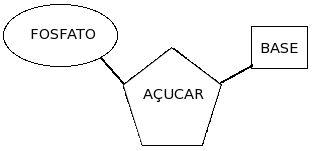
\includegraphics[scale=0.7]{./figuras/componentes_nucleotideo.png}
    \caption{Componentes de um nucleotídeo}
    \label{fig:nucleotideo}
\end{figure}

\begin{figure}[htb!]
    \centering
    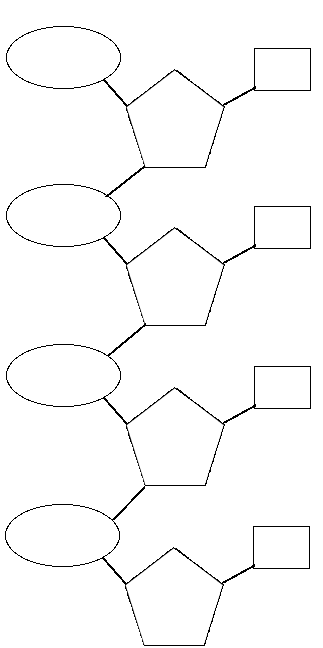
\includegraphics[scale=0.5]{./figuras/sequencia_nucleotideo.png}
    \caption{Sequência linear de nucleotídeos ligados}
    \label{fig:sequencia_nucleotideo}
\end{figure}

Existem duas importantes diferenças entre o RNA e o DNA, que são: o tipo de açúcar e as bases nitrogenadas. O açúcar no DNA é a desoxirribose e no RNA a ribose (Figura \ref{fig:tipos_acucar}). Em cada ácido nucleico são encontradas quatros bases nitrogenadas, sendo que três delas são compartilhadas entre o RNA e DNA são elas: adenina (A), guanina (G) e citosina (C). A base timina (T), é encontrada só no DNA, e a uracila (U), é encontrada só no RNA. Porém existe outra grande diferença entre o RNA e o DNA no nível estrutural. O RNA geralmente existe como uma única sequência de nucleotídeos, enquanto o DNA existe como duas sequências de nucleotídeos pareadas que formam um helicoide, conhecido como dupla hélice. Na Figura \ref{fig:estrutura_DNA_RNA}, podemos observar a estruturas dos dois ácidos. As bases nitrogenadas no DNA estão no interior da hélice, ligadas por pontes de hidrogênio formando pares de bases nitrogenadas (pb). Os únicos pares possíveis no DNA são: A ligado com T e C ligado com G \cite{Zaha2000}.

\begin{figure}[htb!]
    \centering
    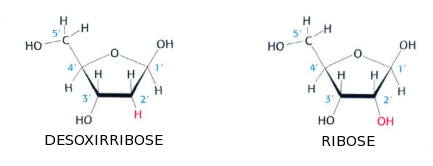
\includegraphics[scale=0.7]{./figuras/tipos_acucar.png}
    \caption{Tipos de açúcar encontrados nos ácidos nucleicos. \cite[Adaptada]{Berg2007})}
    \label{fig:tipos_acucar}
\end{figure}


\begin{figure}[htb!]
    \centering
    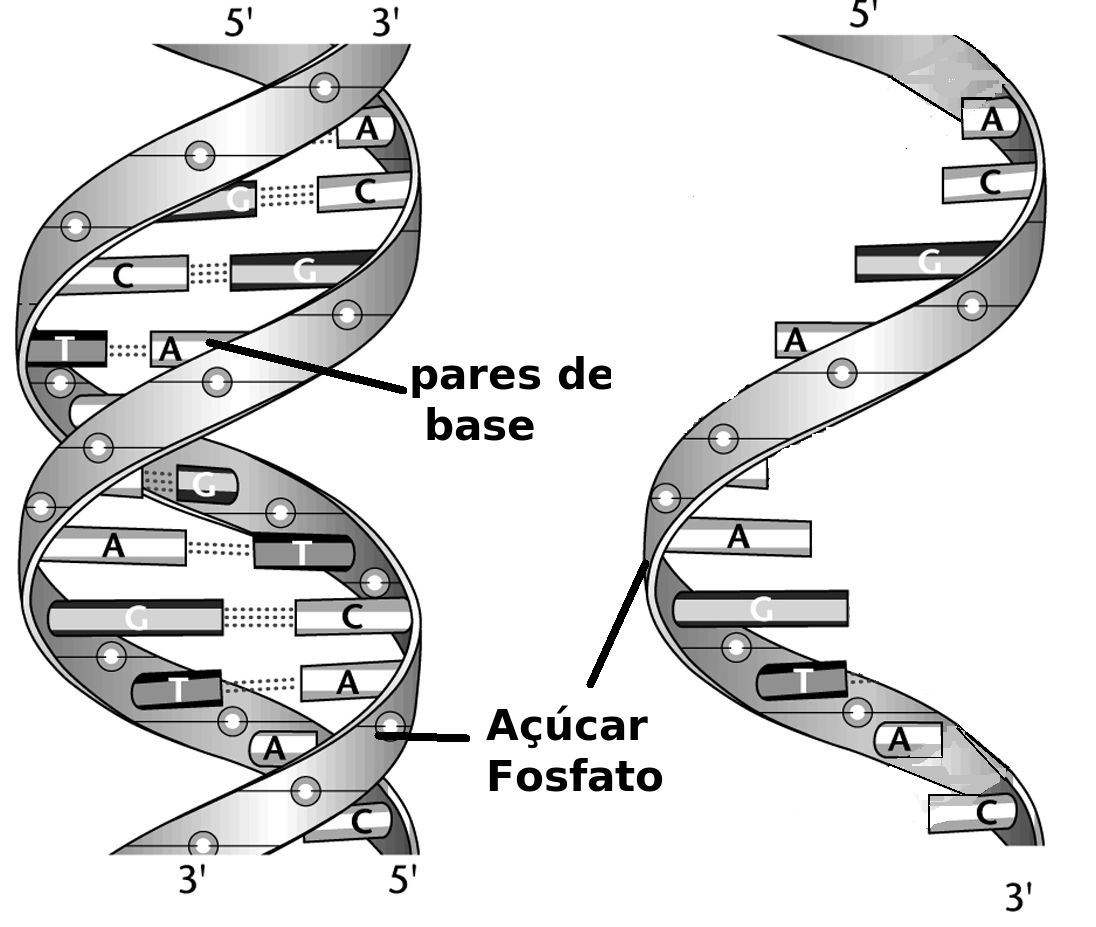
\includegraphics[scale=0.7]{./figuras/estrutura_DNA_RNA.jpg}
    \caption{Estrutura do DNA e RNA. \cite[Adaptada]{Higgs2005}}
    \label{fig:estrutura_DNA_RNA}
\end{figure}

Quanto a estrutura do RNA, ele pode ser dividido em várias classes conforme a sua funcionalidade na célula. A Tabela \ref{T1} mostra as diferentes classes de RNA e suas funcionalidades. 
\begin{table}
\begin{tabularx}{\textwidth}{ |X|X|X|X|X| }    \hline \label{T1}
		  	Classe de RNA      & Função          \\ \hline \hline

    RNA ribossômico (rRNA)  & Componentes estrutural e funcional do ribossomos  \\ \hline
	RNA mensageiro (mRNA)   & Carrega o código genético para a síntese de proteínas\\ \hline
    RNA transportador (tRNA)& Transporta aminoácidos para o mRNA durante a síntese de proteínas \\ \hline
	\textit{Small nuclear RNA} (snRNA)& Processamento do pre-RNA \\ \hline
	\textit{Small nucleolar RNA} (snoRNA)& Processamento e montagem do rRNA \\ \hline
	\textit{Small cytoplasmic RNA} (scRNA)& Variável\\ \hline
	\textit{MicroRNA} (miRNA)& Inibe a tradução do mRNA \\ \hline
	\textit{Small interfering RNA} (siRNA)& Inicia a degradação de outras moléculas de RNA \\ \hline
	\textit{Piwi-interacting RNA} (piRNA)& Pouco sabe-se de sua função\\ \hline					

\end{tabularx}
\caption{Funcionalidades das diferentes classes de moléculas de RNA}
\end{table}
O RNA apesar de ter apenas uma cadeia de nucleotídeos também tem bases complementares. Na síntese de RNA, descrita com mais detalhes na Seção \ref{trans}, as bases que compõem a sequência do RNA são o complemento das bases copiadas do filamento (sequência de nucleotídeos) do DNA modelo, com a substituição de T por U no RNA . As bases complementares no RNA são: A ligado com U e C ligado com G. 


A Figura \ref{fig:repre_sequencia}, mostra uma sequência de DNA e uma de RNA. Elas são comumente representas como uma palavra formada pelo alfabeto (A, G, C, T), para representações de DNA e (A, G, C, U), para representações do RNA. A leitura é feita da esquerda para a direita, no sentido indicado como 5'$\rightarrow$ 3'. Este tipo de representação torna fácil a visualização, assim como a manipulação a nível computacional, sendo amplamente utilizado em métodos \textit{in silico} que envolvem o DNA e o RNA.

\begin{figure}[htb!]
    \centering
    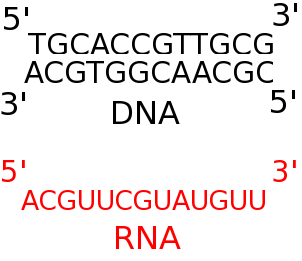
\includegraphics[scale=0.7]{./figuras/repre_sequencia.png}
    \caption{Reapresentação do RNA e DNA}
    \label{fig:repre_sequencia}
\end{figure}

A interação entre o RNA e DNA ocorre quando é necessário a expressão de um gene. Uns dos primeiros passos para a expressão genética é um processo chamado transcrição (Seção \ref{trans}). Neste processo ocorre a formação do RNA (síntese de RNA), a partir de um dos filamentos do DNA. A sequência de RNA formada é uma cópia exata de uma região do RNA. Uma parte desta região que é copiada pertence a um gene. Os genes são seguimentos de DNA podendo ter milhares de pares de bases. São eles que irão especificar o tipo de proteína a ser sintetizado. O processo da síntese de proteínas é conhecido como tradução (Seção \ref{traducao}). A Figura \ref{fig:passo_expresscao_genica}, apresenta cada passo deste conjunto de processos, que também é comumente conhecido como o dogma central.
% talvez falar sobre a importancia da expressão genica

\begin{figure}[htb!]
    \centering
    
\includegraphics[scale=0.7]{./figuras/passo_expresscao_genica.png}
    \caption{Principais passos da expressão de genética}
    \label{fig:passo_expresscao_genica}
\end{figure}

\section{Proteínas}

Proteínas são os componentes principais de todos os seres vivos. Muitas proteínas são enzimas, que atuam como catalizadores biológicos em reações químicas na célula. Outras são componentes estruturais na célula, provendo suporte para membranas, filamentos, ossos, e cabelo. Algumas proteínas ajudam no transporte de substancias, e outras tem funções regulatórias, de comunicação ou de defesa \cite{Pierce2012}.

As proteínas são compostas por uma sequência de aminoácidos. No total são encontrados pelo menos vinte aminoácidos nas proteínas.

Assim como os ácidos nucleicos a estrutura molecular das proteínas tem vários níveis de organização. A primeira estrutura da proteína é a sequência de aminoácidos. A segunda estrutura deriva da interação entre os aminoácidos que faz a estrutura dobrar-se, semelhante ao helicoide do DNA. A terceira estrutura é a forma tridimensional formada pela ligação dos aminácidos na primeira estrutura. A quarta estrutura é a ligação de várias cadeias polipeptídicas\footnote{Cadeias polipeptídicas são cadeias formadas por mais de vinte aminoácidos}. A Figura \ref{fig:estrutura_Proteinas} apresenta as quatro estruturas das proteínas.

\begin{figure}[H]
    \centering
    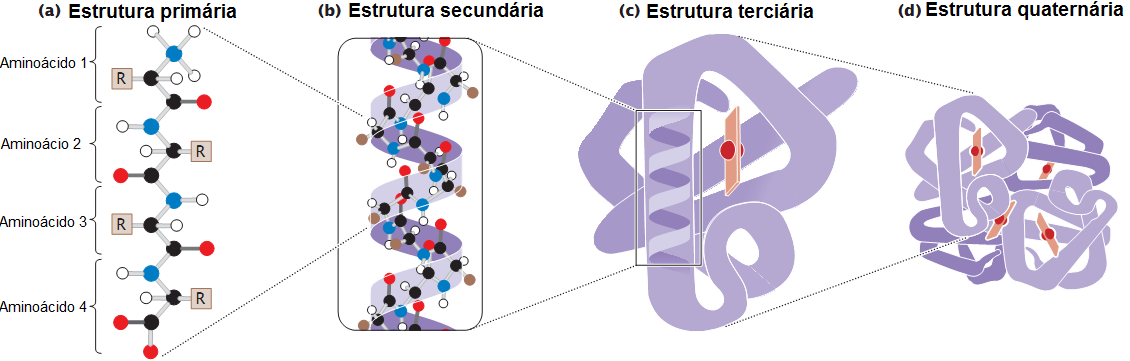
\includegraphics[scale=0.5]{./figuras/estrutura_Proteinas.png}
    \caption{As quatro estruturas das proteínas: (a) A primeira estrutura de uma proteína é sua sequência de aminoácidos; (b) Interações entre aminoácidos faz com que a primeira estrutura se dobre; (c) A segunda estrutura se dobra ainda mais levando a terceira estrutura; (d) Dois ou mais cadeias polipeptídicas associam-se criando a quarta estrutura \cite[Adaptada]{Pierce2012}}
    \label{fig:estrutura_Proteinas}
\end{figure}

\section{Transcrição}\label{trans}

Transcrição é a síntese da molécula de RNA a partir de um molde de DNA. Neste processo uma pequena parte do DNA é copiado. Este tamanho pode variar entre poucos milhares de nucleotídeos, que em comparação com o DNA é muito pequeno, por exemplo uma molécula de DNA no cromossomo humano pode ser maior que 250 milhões de pares de nucleotídeos. Não são todos os genes em uma célula que são transcritos. Porque não é necessário que todas as instruções de funcionamento do organismo seja executada ao mesmo tempo ou na mesma célula \cite{Pierce2012}. A transcrição é um processo altamente seletivo, uma vez que, os genes são transcritos somente quando seus produtos (proteínas) são necessários. Esta seletividade levanta um problema: como reconhecer os genes e transcrevê-los no tempo e local apropriado. 

Para que ocorra a transcrição o primeiro passo é a abertura da hélice dupla do DNA, um dos filamentos do DNA servirá como modelo para a síntese de RNA. A sequência de nucleotídeos na cadeia de RNA é determinada pelo complemento do molde do filamento de DNA (Figura \ref{fig:seq_DNA_molde_e_nao_model}). Qual filamento servirá com molde isso depende do gene que será transcrito. O trecho do DNA que codifica a molécula de RNA e as sequências necessárias para sua transcrição, é chamado de unidade de transcrição. Um complexo de enzimas e proteínas, chamado de aparato de transcrição, reconhece uma unidade de transcrição. Aparece novamente o problema do paragrafo anterior, qual trecho de DNA será lido e como saber o início e a fim dessa leitura. Todas essas informações estão incluídas na sequência do DNA \cite{Pierce2012}. 

Dentro da unidade de transcrição há três regiões: um promotor, uma sequência de codificação do RNA, e um finalizador (Figura \ref{fig:unidade_de_transcricao}). O promotor é uma sequência que o aparato de transcrição reconhece e liga-se. Ele indica qual filamento de DNA será transcrito, em qual direção, e qual é o sítio de início da transcrição (TSS, do inglês \textit{transcription start site}). O TSS é o local onde inicia-se a transcrição, ou seja o primeiro nucleotídeo a ser transcrito. A localização do promotor na unidade de transcrição é antes do TSS e ele não é transcrito em RNA. A segunda região na unidade de transcrição é a sequência de codificação do RNA, a sequência de nucleotídeos de DNA nessa região é transcrita para RNA. A terceira região é o finalizador, uma sequência de nucleotídeos que sinaliza onde é o fim da transcrição. Os finalizadores também fazem parte do RNA, a transcrição para após o finalizador ser copiado \cite{Pierce2012}. Uma definição quanto a direção da transcrição e localização dos nucleotídeos aparece. A direção que o complexo de transcrição se move é chamada de \textit{downstream}, a direção oposta é chamada de \textit{upstream}. Quanto a localização dos nucleotídeos na sequência de DNA, ocorre da seguinte maneira. O primeiro nucleotídeo a ser transcrito (TSS) é numerado com +1, e todos os nucleotídeos localizados \textit{downstream} do TSS são atribuídos números positivos. Nucleotídeos \textit{upstream} do TSS são atribuídos números negativos. Não existe nucleotídeos numerados com 0.


\begin{figure}[H]
    \centering
    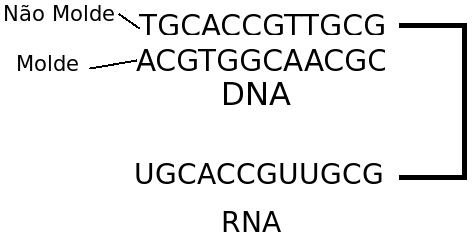
\includegraphics[scale=0.7]{./figuras/seq_DNA_molde_e_nao_model.png}
    \caption{RNA formado, complementar ao filamento modelo}
    \label{fig:seq_DNA_molde_e_nao_model}
\end{figure}

\begin{figure}[H]
    \centering
    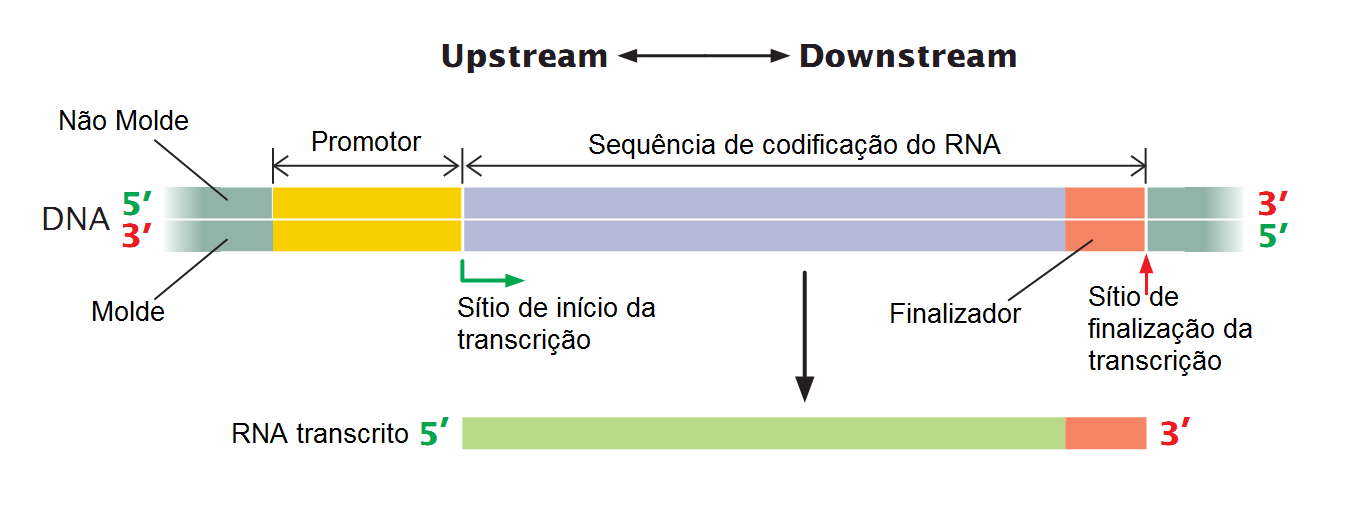
\includegraphics[scale=0.4]{./figuras/unidade_de_transcricao.png}
    \caption{Unidade de transcrição, dividida em promotor, região codificante, e finalizador \cite[Adaptada]{Pierce2012}}
    \label{fig:unidade_de_transcricao}
\end{figure}

Para que ocorra a formação do RNA é necessário a ação de uma enzima que realiza a transcrição, ela é chamada de RNA polimerase. Ela juntamente com proteínas específicas formam o aparato de transcrição. Essas proteínas juntam-se e desconectam-se da RNA polimerase em diferentes níveis no processo de transcrição. Elas atuam como um reforço para a ação da RNA polimerase.

Nos organismos eucarióticos existem três RNA polimerase, chamadas de RNA polimerase I, RNA polimerase II, RNA polimerase III. As três enzimas são similares umas com as outras. A maior diferença entre elas é o tipo de RNA que elas transcrevem:
RNA polimerase I transcreve rRNA; RNA polimerase II transcreve pre-mRNAs, snoRNAs, alguns miRNAs, e alguns snRNAs; e RNA polimerase III transcreve tRNA, pequenos rRNA,alguns miRNAs, e alguns snRNAs (Tabela \ref{TabRNApol}). A RNA polimerase II transcreve a maioria dos genes, ela gera o RNA mensageiro, utilizado na formação das proteínas. 

\begin{table}[H] 
\begin{tabularx}{\textwidth}{ |X|X| }    \hline 
		  	Tipo      & Transcreve\\ \hline \hline

    RNA polimerase I  & grandes rRNAs  \\ \hline
    RNA polimerase II & Pre-mRNA, alguns snRNAs, snoRNAs, alguns miRNAs\\ \hline
    RNA polimerase III & tRNA, pequenos rRNA, snoRNAs, alguns miRNA \\ \hline
\end{tabularx}
\caption{RNA polimerase em eucarióticos \cite[Adaptada]{Pierce2012}}
\label{TabRNApol}
\end{table}

O reconhecimento do promotor é feito por um conjunto de proteínas que ligam-se no promotor para que a RNA polimerase também possa se conectar no promotor. Este conjunto de proteínas pode ser dividido em duas classes. A primeira composta pelos fatores de transcrição gerais, que juntamente com a RNA polimerase formam o aparato basal de transcrição. Este é formado por um grupo de proteínas que se ligam próximo do TSS, ele é suficiente para iniciar a transcrição em seu nível minimo. A outra classe é formada pelos fatores de transcrição específicos que se ligam a específicos segmentos de DNA, aumentando o nível de transcrição pela estimulação do aparato de transcrição na TSS \cite{Pierce2012}. Neste trabalho será apresentado apenas o processo de transcrição com a RNA polimerase II, que transcreve os genes que codificam proteínas. Os promotores encontrados na RNA polimerase II, é dividido em duas partes: promotor principal e promotor regulatório.

O promotor principal está localizado \textit{upstream} do gene e é o local onde o aparato basal de transcrição se conecta. O promotor principal inclui uma ou mais sequências consenso. Por exemplo um sequência consenso comum é a TATA-box, que é formada pela sequência TATAAA e é localizada aproximadamente -25 a -30 pares de base \textit{upstream} do TSS. A Figura \ref{fig:seq_consenso} mostra a TATA-box assim com sequências consensos adicionais.


\begin{figure}[H]
    \centering
    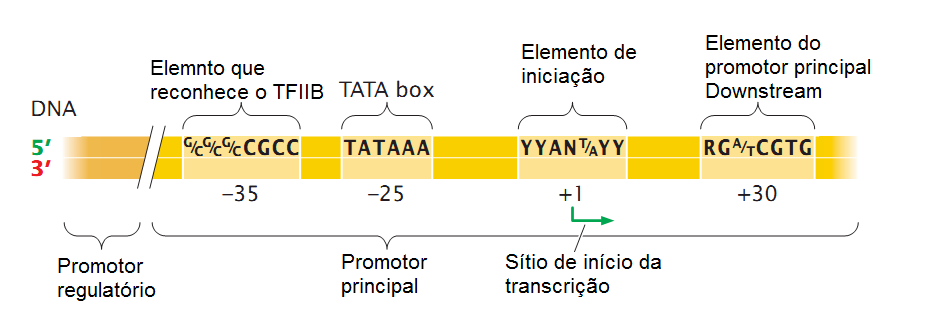
\includegraphics[scale=0.7]{./figuras/seq_consenso.png}
    \caption{Promotor e algumas sequências promotoras, nem todas as sequências mostradas são encontradas em todos os promotores \cite[Adaptada]{Pierce2012}}
    \label{fig:seq_consenso}
\end{figure}

O promotor regulatório é localizado \textit{upstream} do promotor principal. Neste promotor uma variedade de sequências consenso pode ser encontrada. Os fatores de transcrição específicos ligam-se a essas sequências e direto ou indiretamente faz contato com o aparato basal de transcrição, afetando a taxa que a transcrição é iniciada (Figura \ref{fig:promotor_regulacao}). Os fatores de transcrição específicos podem se conectar em sequências distantes chamadas de acentuadores. O DNA entre um acentuador e  promotor forma uma dobra, e os fatores de transcrição ligados no acentuador podem interagir com o aparato de transcrição basal no promotor principal \cite{Simmons2003}.

\begin{figure}[H]
    \centering
    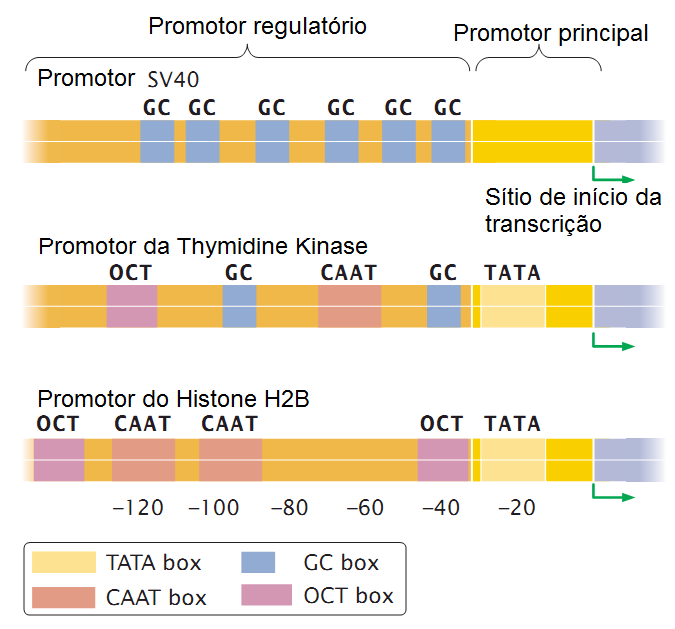
\includegraphics[scale=0.7]{./figuras/promotor_regulacao.png}
    \caption{ Três sequências promotoras de diferentes genes, note como as sequências consenso são ordenadas em diferentes combinações em cada gene\cite[Adaptada]{Pierce2012}}
    \label{fig:promotor_regulacao}
\end{figure}

Os fatores de transcrição gerais que formam o aparato basal de transcrição são: TFIIA, TFIIB, TFIID, TFIIE, TFIIF e TFIIH, onde TF é a sigla para \textit{trancription factor} em inglês, a numeração II indica a RNA polimerase II e a letra identifica um fator de transcrição individual. O complexo formado é apresentado na Figura \ref{fig:iniciacao_trans}. 


\begin{figure}[H]
    \centering
    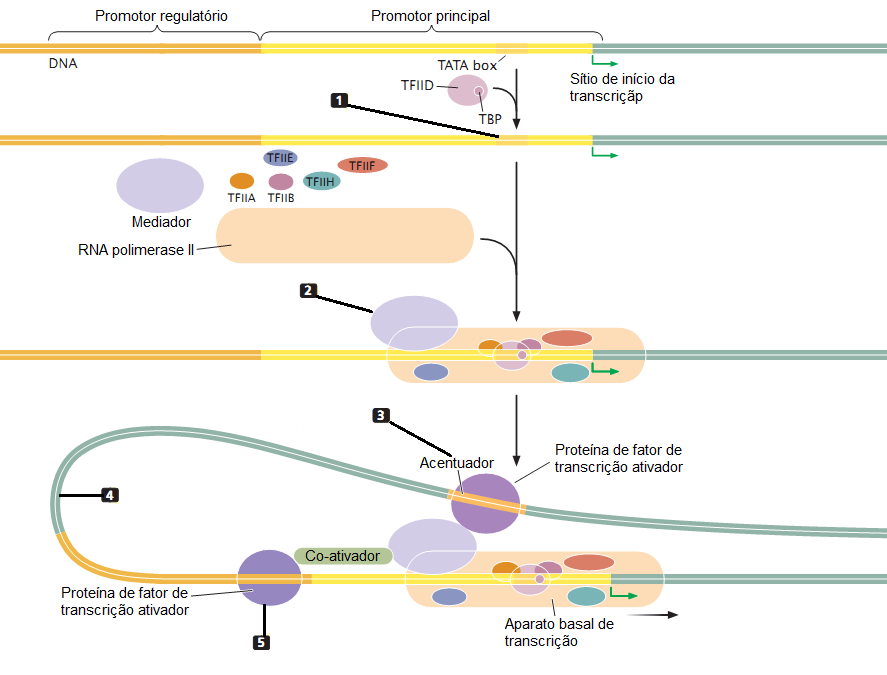
\includegraphics[scale=0.7]{./figuras/iniciacao_trans.png}
    \caption{ Início da transcrição com a RNA polimerase II: (1) TFIID conecta-se na TATA-box no promotor principal; (2) Fatores de transcrição e a RNA polimerase II conectam-se no promotor principal; (3) Proteínas de fator de transcrição específico conectam-se em sequências acentuadoras; (4) DNA faz uma volta, permitindo que proteínas se conectem nos acentuadores para interagir com o aparato basal de transcrição; (5) Proteínas de fatores de transcrição específico conectam-se nas sequências no promotor regulatório e interagem com o aparato basal de transcrição através de um mediador \cite[Adaptada]{Pierce2012}}
    \label{fig:iniciacao_trans}
\end{figure}

O primeiro passo para o inicio da transcrição é o TFIID se conectar na sequência de DNA TATA-box e separar parcialmente os filamentos. Outros fatores de transcrição se conectam em outras sequências consenso no promotor principal, na RNA polimerase e posicionam ela sobre o TSS.

Após a conexão da RNA polimerase e dos fatores de transcrição, formando o aparato de transcrição, a sequência de DNA é separada então a RNA polimerase move-se ao longo do DNA na direção 5' para a 3', deixando o promotor e muitos fatores de transcrição, formando a cadeia de RNA que vai se alongando um nucleotídeo por vez, terminando com uma sequência de nucleotídeos exatamente complementar ao filamento de DNA usado como modelo (Figura \ref{fig:Rnapolimerase}).  Após terminada a cópia a cadeia de RNA, juntamente com a RNA polimerase, se desconectam. A Figura \ref{fig:RNAPOLII} mostra o caminho percorrido da RNA polimerase durante a transcrição.

\begin{figure}[H]
    \centering
    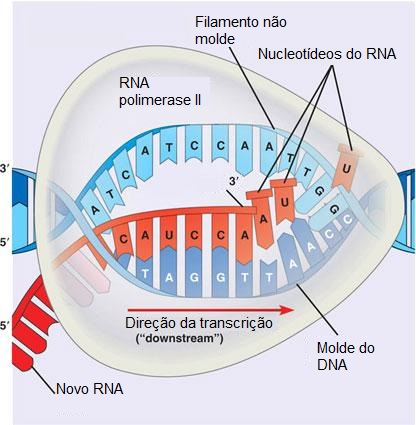
\includegraphics[scale=0.7]{./figuras/RNA-polimerase.jpg}
    \caption{Formação do RNA através da RNA polimerase Fonte: http://www.bio.miami.edu/dana/250/250SS11\_8.html}
    \label{fig:Rnapolimerase}
\end{figure}

\begin{figure}[H]
    \centering
    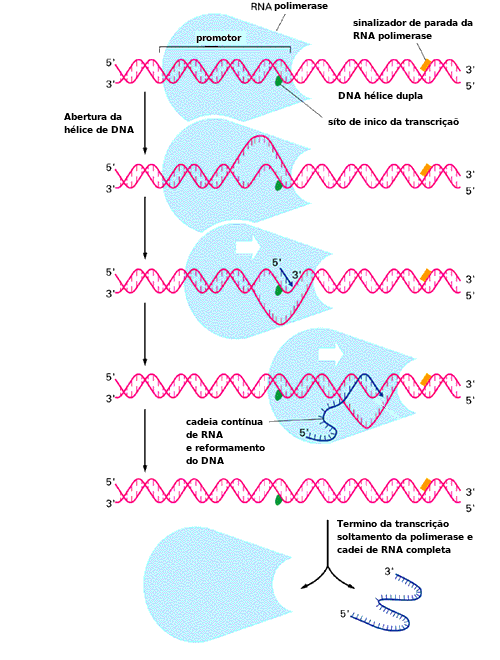
\includegraphics[scale=0.7]{./figuras/RNAPOLII.png}
    \caption{Movimento da RNA polimerase \cite[Adaptada]{Higgs2005}}
    \label{fig:RNAPOLII}
\end{figure}

\section{Código genético}
Como já comentado na Seção \ref{acidos}, a informação codificada no DNA na forma de pares de nucleotídeos é a base para toda a diversidade, funcionalidade, e sobrevivência, nos seres vivos. Para utilizar a informação contida no DNA é necessário decodifica-la. O produto desta decodificação é o código genético.

O código genético é formado a partir da leitura do mRNA, ele é composto por palavras de três nucleotídeos consecutivos. No total são permitidos $4^3 = 64$ possíveis códons \footnote{Códons é a trinca formada pelos nucleotídeos consecutivos}. Sendo que três destes códons são códons finalizadores, especificando o fim da tradução(Seção \ref{traducao}). Os outros 61 códons codificam aminoácidos. Existem vinte aminoácidos mas temos 61 códons para representa-los, isto significa que os aminoácidos são especificado por mais de um códon, com exceção do triptofano e da metionina, que são formados por apenas um códon \cite{Griffiths2000}. Os códons que especificam o mesmo aminoácidos são chamados de sinônimos. A Figura \ref{fig:tab_condos} apresenta os aminoácidos e todos os possíveis códons. Já na Figura \ref{fig:mRNA_to_codon} mostra uma sequência de mRNA decodificada em códons.
 
\begin{figure}[htb!]
    \centering
    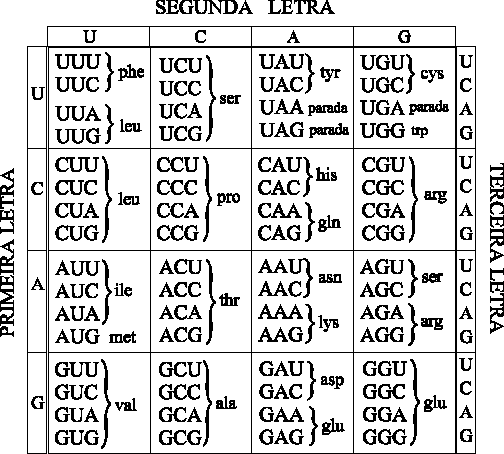
\includegraphics[scale=0.7]{./figuras/tab_condos.png}
    \caption{O código genético formado por 64 códons Fonte: http://www.biomania.com.br/bio/conteudo.asp?cod=1238}
    \label{fig:tab_condos}
\end{figure}

\begin{figure}[htb!]
    \centering
    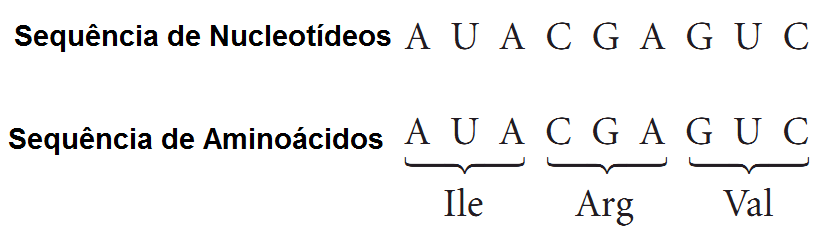
\includegraphics[scale=0.7]{./figuras/mRNA_to_codon.png}
    \caption{Decodificação do mRNA para aminoácidos}
    \label{fig:mRNA_to_codon}
\end{figure}


\section{Tradução} \label{traducao}
A tradução é processo da síntese da proteína a partir do mRNA. Diferente da transcrição a tradução não ocorre núcleo, mas sim no citoplasma da célula onde estão localizados o ribossomos. Os ribossomos são formados de duas subunidades, uma grande e uma pequena. Na tradução mRNA é decodificado para produzir uma sequência de polipeptídeo de acordo com a trinca no código genético. Ou seja utilizando uma cadeia de mRNA será formado a síntese de uma cadeia de aminoácido que por sua vez formará uma proteína \cite{Simmons2003}. O processo da tradução pode ser dividido em quatro partes: 
\begin{enumerate}

\item  \textbf{Ativação}

Um aminoácido é ligado ao complemento de sua trinca no tRNA. Quando há uma ligação entre um aminoácido e um tRNA, este é chamado de "carregado".
\item \textbf{Iniciação}

Nesta etapa os componentes necessários para a tradução são montados no ribossomo, com a ajuda dos fatores de iniciação, que são proteínas que auxiliam o processo.

\item \textbf{Alongamento}

Nesta fase aminoácidos são juntados um por vez. Os tRNA carregados se conetam formando uma sequência de aminoácidos (cadeia polipeptídica).

\item \textbf{Término}

O último processo, na qual a síntese de proteína para em um códon finalizador e os componentes da tradução são soltos do ribossomo.
\end{enumerate}
Durante ou depois deste processo a cadeia de polipeptídeo assumi as estruturas secundária, terciária e quaternária da proteína. A figura \ref{fig:sintese_proteina} resume o processo da tradução.

\begin{figure}[H]
    \centering
    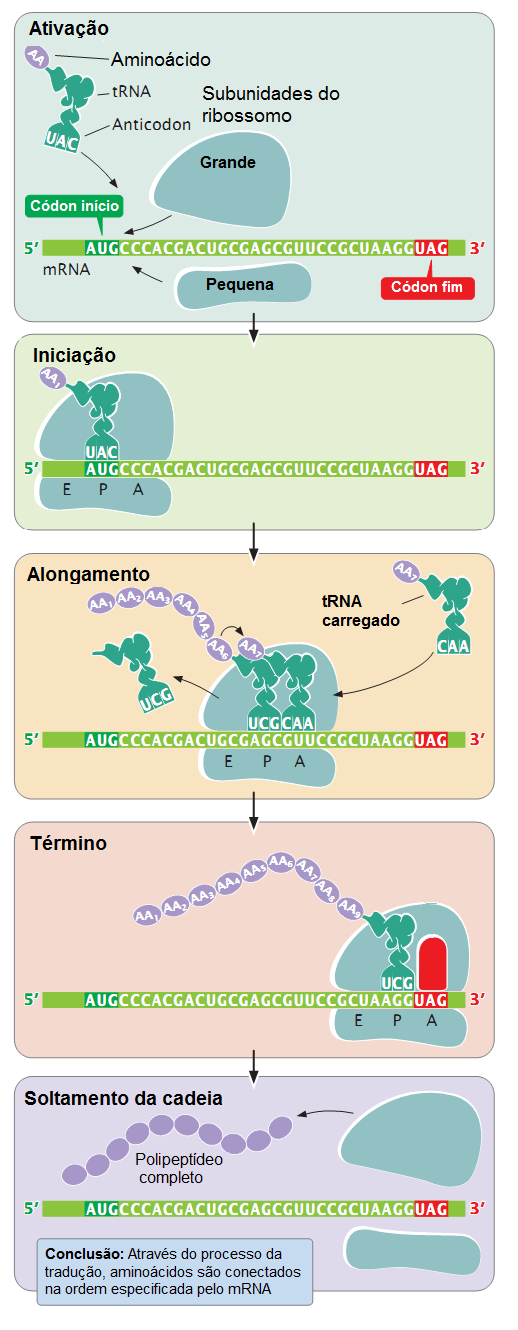
\includegraphics[scale=0.7]{./figuras/sintese_proteina.png}
    \caption{As quatro fases da tradução}
    \label{fig:sintese_proteina}
\end{figure}


\section{Regulação no início da transcrição} \label{S3}

Existem vários níveis de controle da expressão de um gene. Entre estes processão então : a transcrição, alteração da cromatina, alteração da estrutura do DNA, processamento e degradação do RNA, processos que afetam a tradução ou a modificação de proteínas. Nesta seção da continuidade a Seção \ref{trans}, detalhando a ação dos fatores de transcrição específicos, a classificação que os fatores de transcrição recebem segundo suas funções, outras proteínas envolvidas que interagem com eles, e por último genes que têm sua regulação combinada.

Os fatores de transcrição específicos são divididos em duas classes: os ativadores, estimulam a transcrição; e os repressores inibem a transcrição. Os ativadores estimulam e estabilizam o aparato basal de transcrição. Eles podem atuar diretamente com o aparato basal de transcrição ou indiretamente através das proteínas co-ativadoras. Os ativadores podem se conectar em uma sequência de base, geralmente consenso, no promotor regulatório ou em um acentuador. No promotor regulatório há diferentes sequências consenso, em que diferentes fatores ativadores se conectam. Essa sequências consenso são chamadas de elementos regulatórios, e elas podem formar várias combinações (Figura \ref{fig:promotor_regulacao}), então cada promotor é regulado por uma combinação única de fatores de transcrição ativadores \cite{Pierce2012}. Múltiplos elementos de regulatórios formam os CRMs (do inglês, \textit{cis-elements modules}), que integra a conexão de vários fatores de transcrição resultando em um controle combinatório, e em um padrão específico da expressão de um gene \cite{Priest2009}. As funções dos elementos regulatórios e dos CRMs são essenciais as respostas celulares a estímulos \cite{Priest2009}.

A outra classe de fatores de transcrição são os repressores, eles se conectam em elementos regulatórios no promotor regulatório ou em sequências distantes chamadas de silenciadores, que semelhantes aos acentuadores eles são independente de posição e orientação \cite{Pierce2012}. Os repressores competem com os ativadores em três situações:

\begin{enumerate}
\item Se uma região é ocupada por um ativador, a transcrição é ativada, mas se um repressor ocupa o espaço, não há ativação.

\item Um repressor conecta-se próximo a um ativador e impede o ativador interagir com o aparato de transcrição.

\item Um repressor interfere diretamente na montagem do aparato de transcrição, bloqueando a iniciação da transcrição.

\end{enumerate}

\subsection{Regulação combinada}

Alguns genes são ativados pelos mesmos estímulos, eles têm em comum os mesmos elementos regulatórios no promotor ou no acentuador. Estes elementos regulatórios são chamados de elementos de respostas, são sequências pequenas que geralmente têm uma sequência consenso (Tabela \ref{Taq}). Os elementos de resposta são locais de ligação para os fatores de transcrição, que quando ligados aumenta o nível da transcrição. O mesmo elemento de resposta pode estar presente um vários genes permitindo que múltiplos genes sejam ativados pelo mesmo estímulo. Um estímulo pode ser um estresses como mudança na temperatura, mudança hormonal entre outros. Na próxima seção detalharemos um importante fator de transcrição (\textit{dehydration responsive element binding proteins}) que se liga no elemento de resposta \textit{dehydration responsive element}.

\begin{table}[H]
\begin{tabularx}{\textwidth}{ |X|X|X| }    \hline 
		  	Elemento de resposta      & Tipo de resposta & Sequência consenso         \\ \hline \hline

    Heat-shock element & Calor e outros estresses & CNNGAANNTCCNNG \footnote{O \textit{N} no meio da sequência indica que nesta posição pode haver qualquer base} \\ \hline
	Glucocorticoid response element & Glococorticoids & TGGTACAAATGTTCT\\ \hline
    Phorbol ester response element & Phorbal esters & TGACTCA \\ \hline
    Serum response element & Serum & CCATATTAGG \\ \hline
	Dehydration responsive element & mudanças de temperatura, alta salinidade, e seca& A/GCCGAC \footnote{A barra entre as bases A e G, indica que nesta posição pode aparecer tanto A quanto G}\\ \hline

\end{tabularx}
\caption{Alguns elementos de resposta}
\label{Taq}
\end{table}

\section{Dehydration responsive element binding proteins (DREB)}

No amplo conjunto de fatores de transcrição, existem aqueles que quando ligados nos elementos de resposta irão ativar as respostas da célula a estresses abióticos. O estresse abiótico afeta diversos organismos, mas em especial os organismos vegetais que são dependentes de fatores ambientais, são os mais afetados. Nesta seção apresentaremos o \textit{dehydration responsive element binding proteins} (DREB) um importante fator de transcrição nas plantas.

O DREB ativa genes que estão relacionados com a resposta da célula a estímulos abióticos, com a ativação destes genes, a planta se adapta as condições adversas a sua sobrevivência, através de reações bioquímicas e físicas que ocorrem na planta. Os estresses abióticos que mais afetam as plantas são: seca, alta salinidade e mudanças de temperatura. O estresse abiótico atrapalha a sobrevivência e consequentemente a produção de grãos como a soja, arroz, milho e o trigo.

O DREB está contido dentro de uma família de fatores de transcrição única nas plantas, a \textit{Ethylene Responsive Element} (ERF). A ERF desempenha um importante papel em resposta a estímulos abióticos e bióticos. O DREB pode ser dividido em duas subclasses DREB1 e DREB2, envolvidas em estresses de baixa temperaturas e desidratação, respectivamente \cite{Chen2007GmDREB2}.

O elemento de resposta que se conecta no DREB é chamado de \textit{dehydration responsive element} DRE, e ele é formado pela sequência A/GCCGAC \cite{Nakashima2009}. Entretanto para que o DRE seja funcional ele tem que estar acompanhado de elementos regulatórios, mas a especificidade desses elementos regulatórios é baixa, fazendo que muitos desses variem de gene para gene \cite{Zhang2005}. Portanto, em uma busca computacional de genes alvos do DREB (ou outro fator de transcrição), não basta procurar o DRE (ou outro elemento resposta), na região promotora, uma vez que outros elementos regulatórios também participam da regulação, isto torna a busca por genes alvo uma difícil tarefa, uma vez que há uma variação nos elementos regulatórios de um gene para outro.

Segundo \cite{Agarwal2006}, o entendimento do DREB na regulação de um gene é de grande importância para o desenvolvimento de plantas tolerantes a estresses. Já que, estresses abióticos e bióticos influenciam negativamente na sobrevivência e na larga produção de grãos. Culturas como soja, arroz e trigo que são amplamente usadas na alimentação mundial são prejudicadas pelos estresses que muitas vezes impedem uma alta produtividade. 

\chapter{Busca de genes alvos de fatores de transcrição}

Para decifrar a regulação gênica de um organismo, e consequentemente ter um domínio na manipulação genética do organismo, muitas metodologias \textit{in vitro} e \textit{in silico} foram propostas. Das metodologias \textit{in silico}, algumas focam na busca de genes alvos de fatores de transcrição, e outras na classificação da funcionalidade de um gene desconhecido a partir de um gene conhecido, busca de elementos regulatórios, construção da rede de regulação, entre outras. A seguir serão apresentados algumas metodologias para a busca de genes alvos de fatores de transcrição. Esta é uma tarefa importante, porque identificando o fator de transcrição associado ao gene é possível saber qual a funcionalidade do gene. A descoberta da funcionalidade de um gene e quais os fatores de transcrição estão associados com a transcrição deste, tem várias utilidades dependendo do organismo. Por exemplo em uma planta abre a possibilidade de fazer um melhoramentos genético. Em bactérias desenvolver drogas que inibem genes essenciais para a seu desenvolvimento. Existem inúmeras aplicações variando em cada organismo.
%Explicar melhor sobre a importacia da busca de genes alvos aqui no incio antes de falar sobre trabalhos relacionados 

\section{Estado da arte}
Para inferir genes alvos do DREB na \textit{Arabidopsis} \cite{Wang2009}, criaram uma estratégia computacional, que combina a análise de elementos regulatórios e aprendizagem de máquina.

Eles utilizaram como conjunto de dados: sequências da região promotora de genes alvos do DREB identificados experimentalmente, estes são identificados como genes mestres (MGs, do inglês \textit{Master genes}); \textit{DRE frame sequences} (DFSs), fragmentos de DNA com 206 pb (pares de bases), retirados das regiões promotora de MGs, contendo a subsequência consenso (A/GCCGAC) que é a região onde o DREB se conecta em um gene, identificada pelos autores como DRE-motif \footnote{\textit{motif} são regiões conservadas no DNA, assim todos os elementos regulatórios no DNA são \textit{motif}, e não todos os \textit{motifs} são elementos regulatórios}; \textit{Non-DRE frame sequences} (nDFS) fragmentos de DNA com 206 pb, retirados das regiões promotora de gene aleatórios, com um DRE-motif inserido artificialmente na região central. No total foram encontrados 48 DFSs de regiões promotora de MGs, que foram considerados como dados positivos, e 1000 nDFSs como dados negativos.

Após a seleção do conjunto de dados, foi construído um classificador SVM para categorizar DFSs e nDFSs. O vetor de características utilizado no SVM, foi um vetor contendo hexâmeros (pequenos fragmentos de DNA com 6 nucleotídeos), que foram selecionados através do algoritmo HexDiff \cite{Chan2005}. Este algoritmo computa o valor da frequência de um hexâmero no conjunto positivo $F_{p}(h)$ e negativo $F_{n}(h)$ em ambos filamentos de DNA. Depois de calculada a frequência para cada hexâmero em ambos os conjuntos de dados foi calculado o valor da razão $R(h)$, como:
\begin{equation}
R(h) = \frac{F_{p}(h)}{F_{n}(h)}
\end{equation}
Os hexâmeros com a razão maior que um limite estabelecido, foram colocados em um vetor $H_{d}$, que é o vetor de características da SVM. Para cada hexâmero em $H_{d}$ que pertence ao conjunto de DFS foi atribuído o rótulo (+1), e os de nDFS foi atribuído (-1). A função Kernel utilizada no classificador SVM foi a \textit{Radial Basis Function}   (RBF). Para o treinamento do classificador, visto que havia uma disparidade grande entre os dados positivos e negativos, foram usadas apenas 100 amostras negativas e todas as 48 amostras positivas. Já na classificação de DFSs e nDFSs foram utilizadas as 1000 amostras negativas, os dados positivos passaram por um processo de reamostragem, uma vez que eles estavam em um quantidade bem menor (48 DFSs) em relação aos dados negativos, assim o conjunto de dados positivos aumentou para 500 amostras.

Para a previsão de genes alvos do DREB, primeiramente foram selecionados genes em todo o genoma da \textit{Arabidopsis}, cuja a região promotora tem a sequência consenso do DREB (A/GCCGAC). Então foram selecionadas as regiões a esquerda da sequência consenso e a direita, ambas com 100 pb, que juntamente com o consenso forma uma subsequência de 206 pb. O conjunto de dados formado, com o procedimento descrito, foi classificado com o classificador SVM. Foram considerados genes alvos do DREB, todos os gene que contem  pelo menos um DFSs em sua região promotora. No total, 474 genes foram preditos pela SVM e considerados fortes candidatos a serem alvos do DREB.

Segundo os autores, apenas encontrar regiões nos promotores de um gene contendo o consenso DREB, não é suficiente para inferir este gene como alvo do DREB, devido as perdas de características do DRE-motif. Vários estudos, apontam que elementos regulatórios distribuídos na região promotora influenciam na ligação de um fatore de transcrição e seu gene alvo. O que pode ser entendido que, na PR de genes alvos do DREB não somente o DRE-motif mas também outros elementos regulatórios, influenciam na conexão de um DREB na sequência. Estes outros elementos regulatórios agem como auxiliares para promover a conexão do DREB nos genes alvos. Com a utilização do HexDiff é selecionado regiões conservadas, que podem ser partes de elementos regulatórios que influenciam na ação do DREB, portanto um DFS será formado além da região consenso, também por sub-regiões conservadas.

%%%%%%%%%%%%%%%%%%%%%%%%%%%%%%%%%%%%%%%%%%%%%%%%%%%%%%%%%%%%%%%%%%%%%%%%%%%%%%%%%%%%%%%%%%%%%%%%%%%%%%%%%%%%%%%%%%%%%%%%%

%Holloway2008
\cite{Holloway2008} projetaram uma metodologia utilizando aprendizagem de máquina para a predição de genes alvos de fatores de transcrição específicos e análise da rede regulatória do \textit{Saccharomyces cerevisiae}, uma levedura muito utilizada em estudos genéticos por ter um genoma pequeno e simples comparado a outros organismos.

%definir TF no texto base
Para a classificação dos genes alvos de fatores de transcrição, eles utilizaram uma SVM, porque segundo os autores, os conjuntos de dados genômicos têm uma alta dimensionalidade, podendo chegar a milhares ou dezena de milhares de características numéricas para descrever um gene. Assim muitos algoritmos classificadores, podem ter um baixo desempenho com um número alto de características, ao contrário da SVM que tem um bom desempenho com dados de alta dimensionalidade.

% Definir elementos regulatórios no texto base
Como dados de entrada positivo para o treinamento da SVM, foram pegos genes com elementos regulatórios conhecidos, que se ligam a determinados fatores de transcrição que também são conhecidos. Os elementos regulatórios, seus respectivos genes e os fatores de transcrição, foram selecionados por meio de publicações na literatura. O conjunto de entradas negativo, foi escolhido de subconjuntos de genes que têm um alto \textit{p}-valor, consequentemente com uma probabilidade baixa de ter uma ligação nos fatores de transcrição utilizados.

Depois de selecionado o conjunto negativo são construídos 50 classificadores para cada fator de transcrição, utilizando diferentes subamostras do conjunto negativo, com o mesmo tamanho da amostra positiva. É utilizado 50 classificadores para cada fator de transcrição, porque há uma pequena probabilidade de um gene ser associado incorretamente ao conjunto negativo. Com os 50 classificadores este inoportuno é suavizado.

Para a avaliação de cada classificador é usado a abordagem  \textit{leave-one-out cross-validation} (LOOCV), e também as medidas de desempenho: precisão e valor preditivo positivo (PPV, do inglês positive predictive value), que são usadas como média entre os 50 classificadores.

As características do classificador são selecionadas aplicando o algoritmo SVM \textit{recursive feture elimination} (SVM-RFE), que otimiza o vetor \textbf{w} da SVM, para conter componentes altas, que são melhores para separar as classes positivas e negativas de dados. O processo de seleção de características, usando o SVM-RFE, é repetido até atingir o numero desejado de características, que é 1500, este numero é escolhido porque, quando são usadas 1500 características a medida de precisão é aproximadamente 85\%, que é uma precisão consideravelmente boa. Estas características são escolhidas para cada fator de transcrição e são guardadas durante a avaliação dos 50 classificadores. No final obtiveram um grande conjunto de características para um fator de transcrição, lembrando que os elementos desse conjunto são subconjuntos de características. Então foram escolhidos os 40 características com maior valor, de cada subconjunto de características, que foram guardas em uma lista e é contada quantas vezes cada característica apareceu. Esta lista foi rearranjada, posicionando os elementos que tem uma frequência de aparição maior no topo, resultando o conjunto final de características. Essas características inclui um conjunto diverso de dados incluindo sequências promotoras, medidas de expressão de um gene, conservação filogenética de elementos de sequências, sobre-representação de sequências promotoras, temperatura de fusão de promotores, e outras.

O esquema usado para a montagem dos classificadores funciona da seguinte maneira: passo 1, é reunido o conjunto de dados positivos e negativos, totalizando \textit{n}; passo 2, utilizando o LOOCV é pego \textit{n-1} genes para o conjunto de treinamento e 1 para o conjunto de teste; passo 3 então é usado o SVM-RFE para classificar as características no conjunto de treinamento; passo 4 construir um classificador SVM com as 1500 características. Salvar as características; passo 5, classificar o gene deixado de fora do conjunto de treinamento; passo 6 repetir os passos 2-5 até completar o LOOCV. Salvar todas as características; passo 7 calcular as estatísticas de desempenho (precisão, PPV, etc.); passo 8 repetir passos 1-5 50 vezes; último passo, calcular as estatísticas de desempenho final (média da precisão, média do PPV).

Os autores aplicaram este método em 163 fatores de transcrição do \textit{S. cerevisiae}, com os resultados obtidos eles construíram uma rede de regulação que foi disponibilizada em um servidor web (http://cagt10.bu.edu/TFSVM/main.htm), onde é possível consultar quais são os genes alvos de um fator de transcrição, ou quais fatores de transcrição se ligam em um gene.

%%%%%%%%%%%%%%%%%%%%%%%%%%%%%%%%%%%%%%%%%%%%%%%%%%%%%%%%%%%%%%%%%%%%%%%%%%%%%%%%%%%%%%%%%%%%%%%%%%%%%%%%%%%%%%%%%%%%%%%%%


\cite{Lan2007} desenvolveu um método de classificação de genes segundo suas funcionalidades, mais especificamente de genes que estão envolvidos na resposta das plantas a estresses.

Para a classificação dos genes foram desenvolvidos cinco métodos de aprendizado supervisionado, que foram: \textit{Logistic Regression} (LR), \textit{Linear Discriminant Analysis} (LDA), \textit{Quadratic Discriminant Analysis} (QDA), \textit{Naive Bayes} (NB) e \textit{K-Nearest Neighbors} (KNN). Foram escolhidos estes métodos básicos, porque eles requerem pouca computação e os resultados são bons o suficiente para se fazer análises biológicas. Todos os classificadores montados com os métodos, retornam um valor discriminativo para cada gene avaliado. Cada gene é representado por vetor com 290 dimensões cujas as componentes são valores de expressão do gene em 290 condições experimentais. O valor retornado por um classificador tem que ser maior que o limite estabelecido.

O conjunto de dados usado foi extraído de experimentos relacionados com estresses. No total foram 22.746 genes sobre 290 condições experimentais diferentes. Desses 22.746 genes, 11.553 são genes anotados e com suas funções conhecidas, e desses 1.031 respondem à estresses. Os genes anotados formaram o conjunto de dados de treinamento, onde um gene foi considerado positivo se ele foi anotado como um gene de resposta a estresse, e negativo para os demais. Foram 11.193, o total de genes não anotados, estes foram usados para fazer as previsões. Podem haver alguns falsos negativos, visto que genes que não foram descobertas as funcionalidades, são introduzidos no conjunto negativo, entretanto eles podem ser genes de resposta a estresses.

Antes dos dados serem treinados, eles passaram por um pré-processamento, para reduzir a dimensão do conjunto de dados, para que durante o aprendizado supervisionado os dados sejam usados eficientemente. Isto foi feito com o algoritmo \textit{Principal components analysis} (PCA), que mapeia vetores de alta dimensão para um dimensão menor. O PCA aplicado ao conjunto de dados, que originalmente tinha 290 dimensões, reduziu a dimensão para as dimensões de 5, 10, 15, 20, 40 e 100.

Os classificadores foram treinados com todas as dimensões geradas pelo PCA e pela dimensão original com exceção do KNN, no caso do KNN é usado diferentes valores de $K$ na dimensão original, onde $K$ são os $K$ vizinho mais próximos de um gene. Então foi escolhida a dimensão em que cada algoritmo obteve melhores resultados (no caso do KNN o melhor $K$). Os classificadores com a sua melhor dimensão, foram combinados em um só classificador, onde o valor de discriminação do classificador combinado é uma combinação linear dos discriminastes dos classificadores individuais. Como esperado o classificador combinado obteve melhores resultados que os classificadores individuais.

O resultado final da classificação é um conjunto de genes, que podem ser posicionados quanto ao valor discriminante de um gene responder a estresses, ficando os com maiores valores no topo.
%%%%%%%%%%%%%%%%%%%%%%%%%%%%%%%%%%%%%%%%%%%%%%%%%%%%%%%%%%%%%%%%%%%%%%%%%%%%%%%%%%%%%%%%%%%%%%%%%%%%%%%%%%%%%%%%%%%%%%%%%


\cite{Chan2005} desenvolveu o algoritmo HexDiff. Este algoritmo busca agrupamentos de elementos regulatórios, que atuam juntos na regulação de um gene. Um agrupamento de elementos regulatórios é comumente conhecido por CRM (do inglês \textit{cis-regulatory modules}).

O HexDiff é um tipo de algoritmo de aprendizado de máquina, e foi projetado para discriminar dois tipos de sequências de DNA: CRM, e non-CRM(não agrupamento de elementos regulatórios). Para fazer a classificação é necessário um conjunto de dados de treinamentos, que é obtido através de conhecidos CRMs, que são colocados no conjunto positivo de treinamento, os não conhecidos, os non-CRMs, são inseridos no conjunto negativo. Os dados para teste foram pegos de conhecidos CRMs da  \textit{Drosophila}. Foram encontrados 16 genes que, contém um total de 52 CRMs. Após a seleção dos dados foi calculada a frequência de cada hexâmero, no conjunto negativo $f_{p}(h)$ e positivo $f_{n}(h)$, para calcular a razão $R(h)$:
\begin{equation}
R(h) = \frac{F_{p}(h)}{F_{n}(h)}
\end{equation}
Os hexâmeros mais comuns em CRMs do que em  non-CRMs, obtiveram um alto valor de $R(h)$ e foram armazenados no conjunto $H_{d}$. 

Depois de gerado o conjunto $H_{d}$, ele foi usado para classificar cada posição em uma sequência não conhecida como uma sequência CRM e non-CRM. Para fazer a classificação foi construído uma janela na sequência, entre 1000-2000 pb, que a cada rodada movida 1 pb na sequência, e é calculado a pontuação $S_{i}$ para cada posição $i$ da janela na sequência, pelo produto da razão $R(h)$ e o numero de aparições de um hexâmeros $n(h_{d})$ em $H_{d}$ na janela. Qualquer posição que exceder o limite é considerada um CRM.

Para a avaliação foi usado a abordagem  \textit{leave-one-out cross-validation} (LOOCV), onde dos 16 genes encontrados 15 são treinados e 1 é usado como teste, este processo é feito até que todos os 16 genes sejam usados no conjunto de teste. A precisão das previsões do modelo foi medida com a correlação de Matthew. 

Quando aplicado a no-CRMs da \textit{Drosophila}, além dos CRMs já conhecidos serem previstos, outros 10 CRMs foram encontrados e indicados como fortes candidato a CRMs.
%%%%%%%%%%%%%%%%%%%%%%%%%%%%%%%%%%%%%%%%%%%%%%%%%%%%%%%%%%%%%%%%%%%%%%%%%%%%%%%%%%%%%%%%%%%%%%%%%%%%%%%%%%%%%%%%%%%%%%%%%



Outro trabalho foi o de \cite{Zhang2005}, que projetaram uma aplicação para encontrar genes alvos de fatores de transcrição, na \textit{Arabidopsis thaliana} ,que são induzidos por ácido abscísico(ABA, do inglês \textit{abscisic acid}) e por estresses abióticos.

Os dados utilizados foram coletados de uma plantação de \textit{A.thaliana}, que cresceu a uma temperatura de 24ºC durante 10 dias. Algumas mudas foram expostas ao ABA e/ou estresses abióticos, e outras não. Das sequências extraídas do experimento, foram coletadas no total 366 regiões promotoras de genes regulados após a exposição ao ABA e/ou estresses abióticos para análises.

Para encontrar os genes alvos, primeiramente foi calculada a pontuação de cada subsequência de tamanho $w$ em uma determinada sequência, baseado em padrões com relevâncias biológicas (\textit{motifs}) e em um modelo de \textit{background}. Um \textit{motif} $W$ de tamanho $w$ é representado por uma matriz de peso (PMW, do inglês \textit{Position Weight Matrix}), com $PWM \Theta_{W} = (q_{l,b})$, onde $(q_{l,b})$ é a probabilidade de encontrar a base $b$ na posição $i$ do \textit{motif}, já o modelo de \textit{background} é criado utilizando o modelo de Markov. Este modelo calcula a probabilidade de uma base começar na $j-$ésima posição com $P(j|B_{m}) = \prod_{l=1}^wP(b_{j_l-1}|b_{j+l-2}...b_{j+l-l})$, onde $B_{m}$ é a $m-$ésima ordem do modelo de Markov, e $b_{j}$ é a $j-$ésima base da sequência. Também é calculada a probabilidade de uma subsequência ser um \textit{motif} $\Theta_{W}$, utilizando também o modelo de Markov, com $P(j|\Theta_{W}) = \prod_{l=1}^w q_{l,b_{j+l-1}}$, onde $q_{l,b_{j+l-1}}$ é a probabilidade de encontrar a base $b_{j+l-1}$ na posição $l$-ésima de um \textit{motif}. Então foi calculada a \textit{log-ratio} $A_{j,\Theta_{W},B_{m}} = ln\frac{P(j|\Theta)_{W}}{P(j|B_{m})}.$ A pontuação de uma sequência $S$ é feita utilizando dois \textit{motifs} $\Theta_{M}$ e $\Theta_{N}$ , neste caso um deles é o ABRE que é o elemento de resposta alvo, quando uma planta é exposta ao ABE, são consideradas todas as posições $i$ e $j$ dentro de $S$ e a combinação da pontuação das posições é computada como $A_{S,\Theta_{M},\Theta_{N},B_{m}} = max_{i,j}(A_{i,\Theta_{M},B_{m}} + A_{j,\Theta_{N},B_{m}})$. A combinação com maior pontuação é atribuída para a sequência, genes com sua sequência com maior pontuação têm uma probabilidade maior de serem genes alvos.

Como resultados foram encontrados entre 1825 genes induzidos a estresses, 1530 onde pelo menos uma funcionalidade poderia ser atribuída. E foram selecionados 150 com maior pontuação onde 126 estão classificados em alguma categoria funcionalidade. O que levou aos autores a concluir que podem existir muitas atividades de regulações genicas após a exposição ao ABA.

%%%%%%%%%%%%%%%%%%%%%%%%%%%%%%%%%%%%%%%%%%%%%%%%%%%%%%%%%%%%%%%%%%%%%%%%%%%%%%%%%%%%%%%%%%%%%%%%%%%%%%%%%%%%%%%%%%%%%%%%%


\cite{Bigelow2004CisOrtho} desenvolveram o software CisOrtho , que identifica alvos de fatores de transcrição, com um elemento regulatório definido, utilizando rastros filogenéticos. O programa foi usado nos genomas de dois invertebrados, o \textit{Caenorhabditis elegans} e o \textit{Caenorhabditis briggsae}.

O primeiro passo foi, identificar, classificar, e associar as regiões não codificantes dos genes, isto foi feito com as informações contidas em arquivos GFF (do inglês, \textit{General Feature Format}) extraídos de bancos de dados públicos. Foram retiradas as regiões codificantes porque é improvável que há elementos regulatórios nestas regiões e por elas serem impróprias para buscas filogenéticas apresentando uma alta conservação. O segundo passo consistiu em construir uma PWM (do inglês, \textit{Position Weight Matrix}) para um conjunto de elementos regulatórios definidos experimentalmente, neste trabalho foram usados os elementos regulatórios dos fatores de transcrição TTX-3 e CEH-10. Para a construção da PWM foi usado o software HMMER \cite{Eddy1998}, este software utiliza o modelo oculto de Markov para gerar a PWM. A PWM resultante é usada como entrada no CisOrtho, que faz uma busca nas sequências não codificantes, atribuindo uma pontuação para cada bloco de subsequência de tamanho $n$ (chamado de janela), onde o objetivo é encontrar subsequências com a maior pontuação $N$, e com no máximo $D$ subsequências, onde $N$ e $D$ são definidos pelo usuário. No quarto passo foi feita a análise filogenética, foram utilizados conjuntos de mapeamentos ortólogos\footnote{Sequências conservadas de diferentes organismo, que tem o mesmo ancestral} entre \textit{C. elegans} e \textit{C. briggasae} que provê pares de subsequências ortólogas\footnote{sequências derivadas de um mesmo ancestral}. Os pares de subsequências que apresentam uma alta pontuação são guardados, como um par de subsequência. O último passo classifica os pares de subsequências  de acordo com as suas pontuações e \textit{mismatches}\footnote{Bases diferentes, em uma mesma posição, neste caso é comparado as bases do \textit{C. elegans} e \textit{C. briggasae}}.

Com o CisOrtho foi possível identificar novos genes alvos dos fatores de transcrição TTX-3 e CEH-10, foram encontrados 14 genes com subsequências com alta pontuação que satisfaziam os critérios para serem alvos de TTX-3/CEH-10, também foram encontrados genes com baixa pontuação, mas que atendiam os critérios para serem alvos de TTX-3/CEH-10, um total de 11 genes. Para subsequência com uma grande conservação mas, com uma baixa pontuação, foram feitas análises e foram encontrados também genes alvos.




%%%%%%%%%%%%%%%%%%%%%%%%%%%%%%%%%%%%%%%%%%%%%%%%%%%%%%%%%%%%%%%%%%%%%%%%%%%%%%%%%%%%%%%%%%%%%%%%%%%%%%%%%%%%%%%%%%%%%%%%%
\section{Tabela comparativa}


\begin{tabularx}{\textwidth}{ |X|X|X|X|X| }    \hline
		  Trabalho	   & Organismo    & Entradas     & Técnicas usadas & Resultados obtidos       \\ \hline \hline	

    \cite{Wang2009}     	 &  \textit{Arabidopsis} & sequências promotoras de genes que contém o DRE-motif e sequências que não contém o DRE-motif  & O algoritmo HexDiff e SVM & 474 genes alvos  \\ \hline
    \cite{Holloway2008} 	   & \textit{Saccharomyces cerevisiae}  & sequências promotoras; medidas de expressão de um gene; conservação filogenética de elementos de sequências; sobre-representação de sequências promotoras; temperatura de fusão de promotores; K-mer conservados; k-mer com \textit{mismatches}; \textit{k-mer median position} & SVM & rede de regulação do \textit{Saccharomyces cerevisiae}\\ \hline

\end{tabularx}



\begin{tabularx}{\textwidth}{ |X|X|X|X|X| }    \hline
		  	Trabalho      & Organismo    & Entradas     & Técnicas usadas & Resultados obtidos       \\ \hline \hline

    \cite{Lan2007}     		   & \textit{Arabidopis thaliana}  & 22.746 genes sobre 290 condições experimentais diferentes   & \textit{Logistic Regression} (LR), \textit{Linear Discriminant Analysis} (LDA), \textit{Quadratic Discriminant Analysis} (QDA), \textit{Naive Bayes} (NB) e \textit{K-Nearest Neighbors} (KNN)& Genes com grandes possibilidades de serem expressos mediante a condições de estresses abióticos \\ \hline
    \cite{Chan2005}            & \textit{Drosophila}  & CRM e não-CRM   & HexDiff & 10 novos CRMs\\ \hline
    \cite{Zhang2005}           & \textit{Arabidopsis thaliana}  & dados de plantas expostas ao ABA e/ou estresses abióticos & PWM e modelo de Markov & 1530 genes que pode ser adicionada alguma funcionalidade \\ \hline
    \cite{Bigelow2004CisOrtho} & \textit{Caenorhabditis elegans} e o \textit{Caenorhabditis briggsae}  & arquivos GFF e conjuntos de mapeamentos ortólogos  & Modelo oculto de Markov, PWM e rastros filogenéticos & mais de 25 genes alvos de TTX-3 e CEH-10  \\ \hline           

\end{tabularx}

\section{Discussão}

Podemos observar que a maioria dos trabalhos realizados na busca de genes alvos de fatores de transcrição, estão em comum acordo quanto a degeneração dos elementos regulatórios, e a dependência de um elemento regulatório de outros elementos regulatórios para a regulação de um gene formando os CRMs. Essas observações foram comprovadas em experimentos \textit{in vitro}, como visto em \cite{Davidson1983},\cite{Priest2009} e \cite{Zhang2005}. 

Observamos o importante papel que algoritmos de aprendizado de máquina tem na busca de genes alvos, estes algoritmos são usados em pelo menos uma das etapas das metodologias apresentadas. Em \cite{Holloway2008} e \cite{Lan2007}, é discutido que os dados genômicos apresentam uma alta dimensionalidade, o que nos leva a concluir que a predominância do SVM nas metodologias é devido a facilidade que SVM tem em lidar com alta dimensionalidades e os bons resultados obtidos mediante estas condições.

Quanto a uma análise de desempenho e precisão entre os algoritmos fica inconclusiva, uma vez que os trabalhos foram feitos em diferentes tipos de organismos, mesmo os trabalhos em que os organismo eram os mesmos, eles eram aplicados a diferentes tipos de fatores de transcrição.

Finalizando, é de grande importância descobrir os genes alvos de fatores de transcrição, uma vez que, ainda existem vários genes que ainda não foi associada nenhuma função. Como a função de um gene está diretamente ligada ao tipo de fatores de transcrição que conectam nele, é possível classificar estes genes a partir de fatores de transcrição conhecidos.

\bibliographystyle{abnt-alf}
\bibliography{./arquivos/bibliografia}
\end{document}